% Options for packages loaded elsewhere
\PassOptionsToPackage{unicode}{hyperref}
\PassOptionsToPackage{hyphens}{url}
\PassOptionsToPackage{dvipsnames,svgnames,x11names}{xcolor}
%
\documentclass[
  sn-mathphys-num,
]{sn-jnl}



\usepackage{amsmath,amssymb}
\usepackage{iftex}
\ifPDFTeX
  \usepackage[T1]{fontenc}
  \usepackage[utf8]{inputenc}
  \usepackage{textcomp} % provide euro and other symbols
\else % if luatex or xetex
  \usepackage{unicode-math}
  \defaultfontfeatures{Scale=MatchLowercase}
  \defaultfontfeatures[\rmfamily]{Ligatures=TeX,Scale=1}
\fi
\usepackage{lmodern}
\ifPDFTeX\else  
    % xetex/luatex font selection
\fi
% Use upquote if available, for straight quotes in verbatim environments
\IfFileExists{upquote.sty}{\usepackage{upquote}}{}
\IfFileExists{microtype.sty}{% use microtype if available
  \usepackage[]{microtype}
  \UseMicrotypeSet[protrusion]{basicmath} % disable protrusion for tt fonts
}{}
\makeatletter
\@ifundefined{KOMAClassName}{% if non-KOMA class
  \IfFileExists{parskip.sty}{%
    \usepackage{parskip}
  }{% else
    \setlength{\parindent}{0pt}
    \setlength{\parskip}{6pt plus 2pt minus 1pt}}
}{% if KOMA class
  \KOMAoptions{parskip=half}}
\makeatother
\usepackage{xcolor}
\setlength{\emergencystretch}{3em} % prevent overfull lines
\setcounter{secnumdepth}{-\maxdimen} % remove section numbering
% Make \paragraph and \subparagraph free-standing
\makeatletter
\ifx\paragraph\undefined\else
  \let\oldparagraph\paragraph
  \renewcommand{\paragraph}{
    \@ifstar
      \xxxParagraphStar
      \xxxParagraphNoStar
  }
  \newcommand{\xxxParagraphStar}[1]{\oldparagraph*{#1}\mbox{}}
  \newcommand{\xxxParagraphNoStar}[1]{\oldparagraph{#1}\mbox{}}
\fi
\ifx\subparagraph\undefined\else
  \let\oldsubparagraph\subparagraph
  \renewcommand{\subparagraph}{
    \@ifstar
      \xxxSubParagraphStar
      \xxxSubParagraphNoStar
  }
  \newcommand{\xxxSubParagraphStar}[1]{\oldsubparagraph*{#1}\mbox{}}
  \newcommand{\xxxSubParagraphNoStar}[1]{\oldsubparagraph{#1}\mbox{}}
\fi
\makeatother


\providecommand{\tightlist}{%
  \setlength{\itemsep}{0pt}\setlength{\parskip}{0pt}}\usepackage{longtable,booktabs,array}
\usepackage{calc} % for calculating minipage widths
% Correct order of tables after \paragraph or \subparagraph
\usepackage{etoolbox}
\makeatletter
\patchcmd\longtable{\par}{\if@noskipsec\mbox{}\fi\par}{}{}
\makeatother
% Allow footnotes in longtable head/foot
\IfFileExists{footnotehyper.sty}{\usepackage{footnotehyper}}{\usepackage{footnote}}
\makesavenoteenv{longtable}
\usepackage{graphicx}
\makeatletter
\def\maxwidth{\ifdim\Gin@nat@width>\linewidth\linewidth\else\Gin@nat@width\fi}
\def\maxheight{\ifdim\Gin@nat@height>\textheight\textheight\else\Gin@nat@height\fi}
\makeatother
% Scale images if necessary, so that they will not overflow the page
% margins by default, and it is still possible to overwrite the defaults
% using explicit options in \includegraphics[width, height, ...]{}
\setkeys{Gin}{width=\maxwidth,height=\maxheight,keepaspectratio}
% Set default figure placement to htbp
\makeatletter
\def\fps@figure{htbp}
\makeatother

%%%% Standard Packages

\usepackage{graphicx}%
\usepackage{multirow}%
\usepackage{amsmath,amssymb,amsfonts}%
\usepackage{amsthm}%
\usepackage{mathrsfs}%
\usepackage[title]{appendix}%
\usepackage{xcolor}%
\usepackage{textcomp}%
\usepackage{manyfoot}%
\usepackage{booktabs}%
\usepackage{algorithm}%
\usepackage{algorithmicx}%
\usepackage{algpseudocode}%
\usepackage{listings}%

%%%%

\raggedbottom
\usepackage{multirow}
\usepackage{centernot}
\makeatletter
\@ifpackageloaded{caption}{}{\usepackage{caption}}
\AtBeginDocument{%
\ifdefined\contentsname
  \renewcommand*\contentsname{Table of contents}
\else
  \newcommand\contentsname{Table of contents}
\fi
\ifdefined\listfigurename
  \renewcommand*\listfigurename{List of Figures}
\else
  \newcommand\listfigurename{List of Figures}
\fi
\ifdefined\listtablename
  \renewcommand*\listtablename{List of Tables}
\else
  \newcommand\listtablename{List of Tables}
\fi
\ifdefined\figurename
  \renewcommand*\figurename{Figure}
\else
  \newcommand\figurename{Figure}
\fi
\ifdefined\tablename
  \renewcommand*\tablename{Table}
\else
  \newcommand\tablename{Table}
\fi
}
\@ifpackageloaded{float}{}{\usepackage{float}}
\floatstyle{ruled}
\@ifundefined{c@chapter}{\newfloat{codelisting}{h}{lop}}{\newfloat{codelisting}{h}{lop}[chapter]}
\floatname{codelisting}{Listing}
\newcommand*\listoflistings{\listof{codelisting}{List of Listings}}
\makeatother
\makeatletter
\makeatother
\makeatletter
\@ifpackageloaded{caption}{}{\usepackage{caption}}
\@ifpackageloaded{subcaption}{}{\usepackage{subcaption}}
\makeatother

\ifLuaTeX
  \usepackage{selnolig}  % disable illegal ligatures
\fi
\usepackage{bookmark}

\IfFileExists{xurl.sty}{\usepackage{xurl}}{} % add URL line breaks if available
\urlstyle{same} % disable monospaced font for URLs
\hypersetup{
  pdftitle={A mixture of hidden Markov models to predict the lymphatic spread in head and neck cancer depending on primary tumor location},
  colorlinks=true,
  linkcolor={blue},
  filecolor={Maroon},
  citecolor={Blue},
  urlcolor={Blue},
  pdfcreator={LaTeX via pandoc}}


\title[A mixture of hidden Markov models to predict the lymphatic spread
in head and neck cancer depending on primary tumor location]{A mixture
of hidden Markov models to predict the lymphatic spread in head and neck
cancer depending on primary tumor location}

% author setup
\author[1,2]{\fnm{Yoel Perez} \sur{Haas}}\email{yoel.perezhaas@usz.ch}\author*[1,2]{\fnm{Roman} \sur{Ludwig}}\email{roman.ludwig@usz.ch}\author[1,2]{\fnm{Julian} \sur{Brönnimann}}\author[1,2]{\fnm{Esmée Lauren} \sur{Looman}}\author[2]{\fnm{Panagiotis} \sur{Balermpas}}\author[11]{\fnm{Sergi} \sur{Benavente}}\author[3,4,7]{\fnm{Adrian} \sur{Schubert}}\author[8]{\fnm{Dorothea} \sur{Barbatei}}\author[8]{\fnm{Laurence} \sur{Bauwens}}\author[2]{\fnm{Jean-Marc} \sur{Hoffmann}}\author[3]{\fnm{Olgun} \sur{Elicin}}\author[6,10]{\fnm{Matthias} \sur{Dettmer}}\author[2]{\fnm{Bertrand} \sur{Pouymayou}}\author[4,5]{\fnm{Roland} \sur{Giger}}\author[8]{\fnm{Vincent} \sur{Grégoire}}\author[1,2]{\fnm{Jan} \sur{Unkelbach}}\email{jan.unkelbach@usz.ch}
% affil setup
\affil[1]{\orgdiv{Department of Physics}, \orgname{University of
Zurich}}
\affil[2]{\orgdiv{Radiation Oncology}, \orgname{University Hospital
Zurich}}
\affil[3]{\orgdiv{Department of Radiation Oncology}, \orgname{Bern
University Hospital}}
\affil[4]{\orgdiv{Department of ENT, Head \& Neck
Surgery}, \orgname{Bern University Hospital}}
\affil[5]{\orgdiv{Head and Neck Anticancer Center}, \orgname{Bern
University Hospital}}
\affil[6]{\orgdiv{Institute of Tissue Medicine and
Pathology}, \orgname{Bern University Hospital}}
\affil[7]{\orgdiv{Department of ENT, Head \& Neck
Surgery}, \orgname{Réseau Hospitalier Neuchâtelois}}
\affil[8]{\orgdiv{Department of Radiation Oncology}, \orgname{Centre
Léon Bérard}}
\affil[9]{\orgdiv{Department of Head and Neck Surgery}, \orgname{Centre
Léon Bérard}}
\affil[10]{\orgdiv{Institute of Pathology}, \orgname{Klinikum
Stuttgart}}
\affil[11]{\orgdiv{Departement of Radiation Oncology}, \orgname{Hospital
Vall d'Hebron}}

% abstract 

\abstract{Purpose: to be done

Methods: to be done

Results: to be done

Conclusions: to be done}

% keywords

\begin{document}
\maketitle


\section{Introduction}\label{introduction}

Head and neck squamous cell carcinomas (HNSCCs) are known to spread
through the lymphatic system often leading to metastases in the lymph
nodes \citep{mukherji_cervical_2001, shah_patterns_1990}. To minimize
nodal recurrences, lymph node levels (LNLs) at risk of harboring occult
metastases are typically irradiated electively. Current guidelines for
different tumor locations are based on the overall prevalence of nodal
disease as reported in literature
\citep{biau_selection_2019, mukherji_cervical_2001, shah_patterns_1990}.

To personalize the prediction of the risk of occult metastases, given a
patient's individual diagnosis, we previously published a large,
multi-centric dataset where the lymphatic involvement per LNL is
available for each
patient\citep{ludwig_dataset_2022, ludwig_multi-centric_2023}. Building
on this dataset, we introduced an interpretable hidden Markov model
(HMM), trained to predict the risk for occult nodal disease, given an
individual patient's diagnosis \citep{ludwig_hidden_2021}.

Personalized risk predictions could enable clinicians to safely reduce
the elective clinical target volume (CTV-N), potentially decreasing
treatment-related side effects that impair a patient's quality of life,
without compromising the efficacy of the treatment
\citep{batth_practical_2014}.

Initially, separate models were trained for distinct tumor locations,
such as the oropharynx and oral cavity. These tumor locations are also
used in guidelines to define the elective target volumes
\citep{biau_selection_2019}. However, this approach did not account for
variations in lymphatic spread between subsites within these tumor
regions. With data from more than 2700 patients available, we can now
further analyze subsite specific spread patterns. Closer analysis showed
that pooling subsites into a single model led to inaccurate predictions,
as it failed to capture distinct lymphatic spread patterns. To resolve
this, we propose using a mixture of HMMs, which allows us to model the
lymphatic spread more accurately for tumors located near anatomical
borders, such as those between the oropharynx and oral cavity (e.g.,
tumors in the palate).

Additionally, we extend the analysis to a broader mixture model that
encompasses tumors of the oral cavity, oropharynx, hypopharynx, and
larynx, resulting in further personalized predictions of lymphatic
spread across these regions.

\section{Data on Lymphatic Progression Patterns}\label{sec-data}

For the analyses in this work, we used seven datasets from 5
institutions resulting in 2437 patients in total.

\begin{enumerate}
\def\labelenumi{\arabic{enumi}.}
\tightlist
\item
  287 oropharyngeal patients from the University of Zurich in
  Switzerland
\item
  263 oropharyngeal patients from the Centre Léon Bérard in France
\item
  327 oropharyngeal, larynx and oral cavity patients from the
  Inselspital Bern in Switzerland
\item
  276 oropharyngeal, larynx and oral cavity patients from the Centre
  Léon Bérard in France
\item
  273 oropharyngeal, larynx and oral cavity patients from the University
  of Zurich in Switzerland
\item
  164 oropharyngeal patients from the Hospital Vall d'Hebron in Spain
  (not yet public)
\item
  847 hypopharynx, larynx and oral cavity patients from University
  Medical Center Groningen (not yet public)
\end{enumerate}

Patients with glottic laryngeal cancer (C32.0) at tumor stages T0 and T1
have been excluded from analysis because these stages, by definition, do
not exhibit lymphatic involvement {[}need source from Panos{]}. The
datasets 1-4 are publicly available as CSV tables
\citep{ludwig_multi-centric_2023, ludwig_detailed_2022} and can be
interactively explored on \href{https://lyprox.org}{LyProX}. For each
patient the primary tumor subsite is reportd and each indicidual LNL is
reported as either metastatic or healthy given the available diagnostic
modalities, which include pathology after neck dissection in some
patients. In this work we will stratify the tumor locations into
different ICD codes which are depicted in figure~\ref{fig-subsites}.

\begin{figure}

\centering{

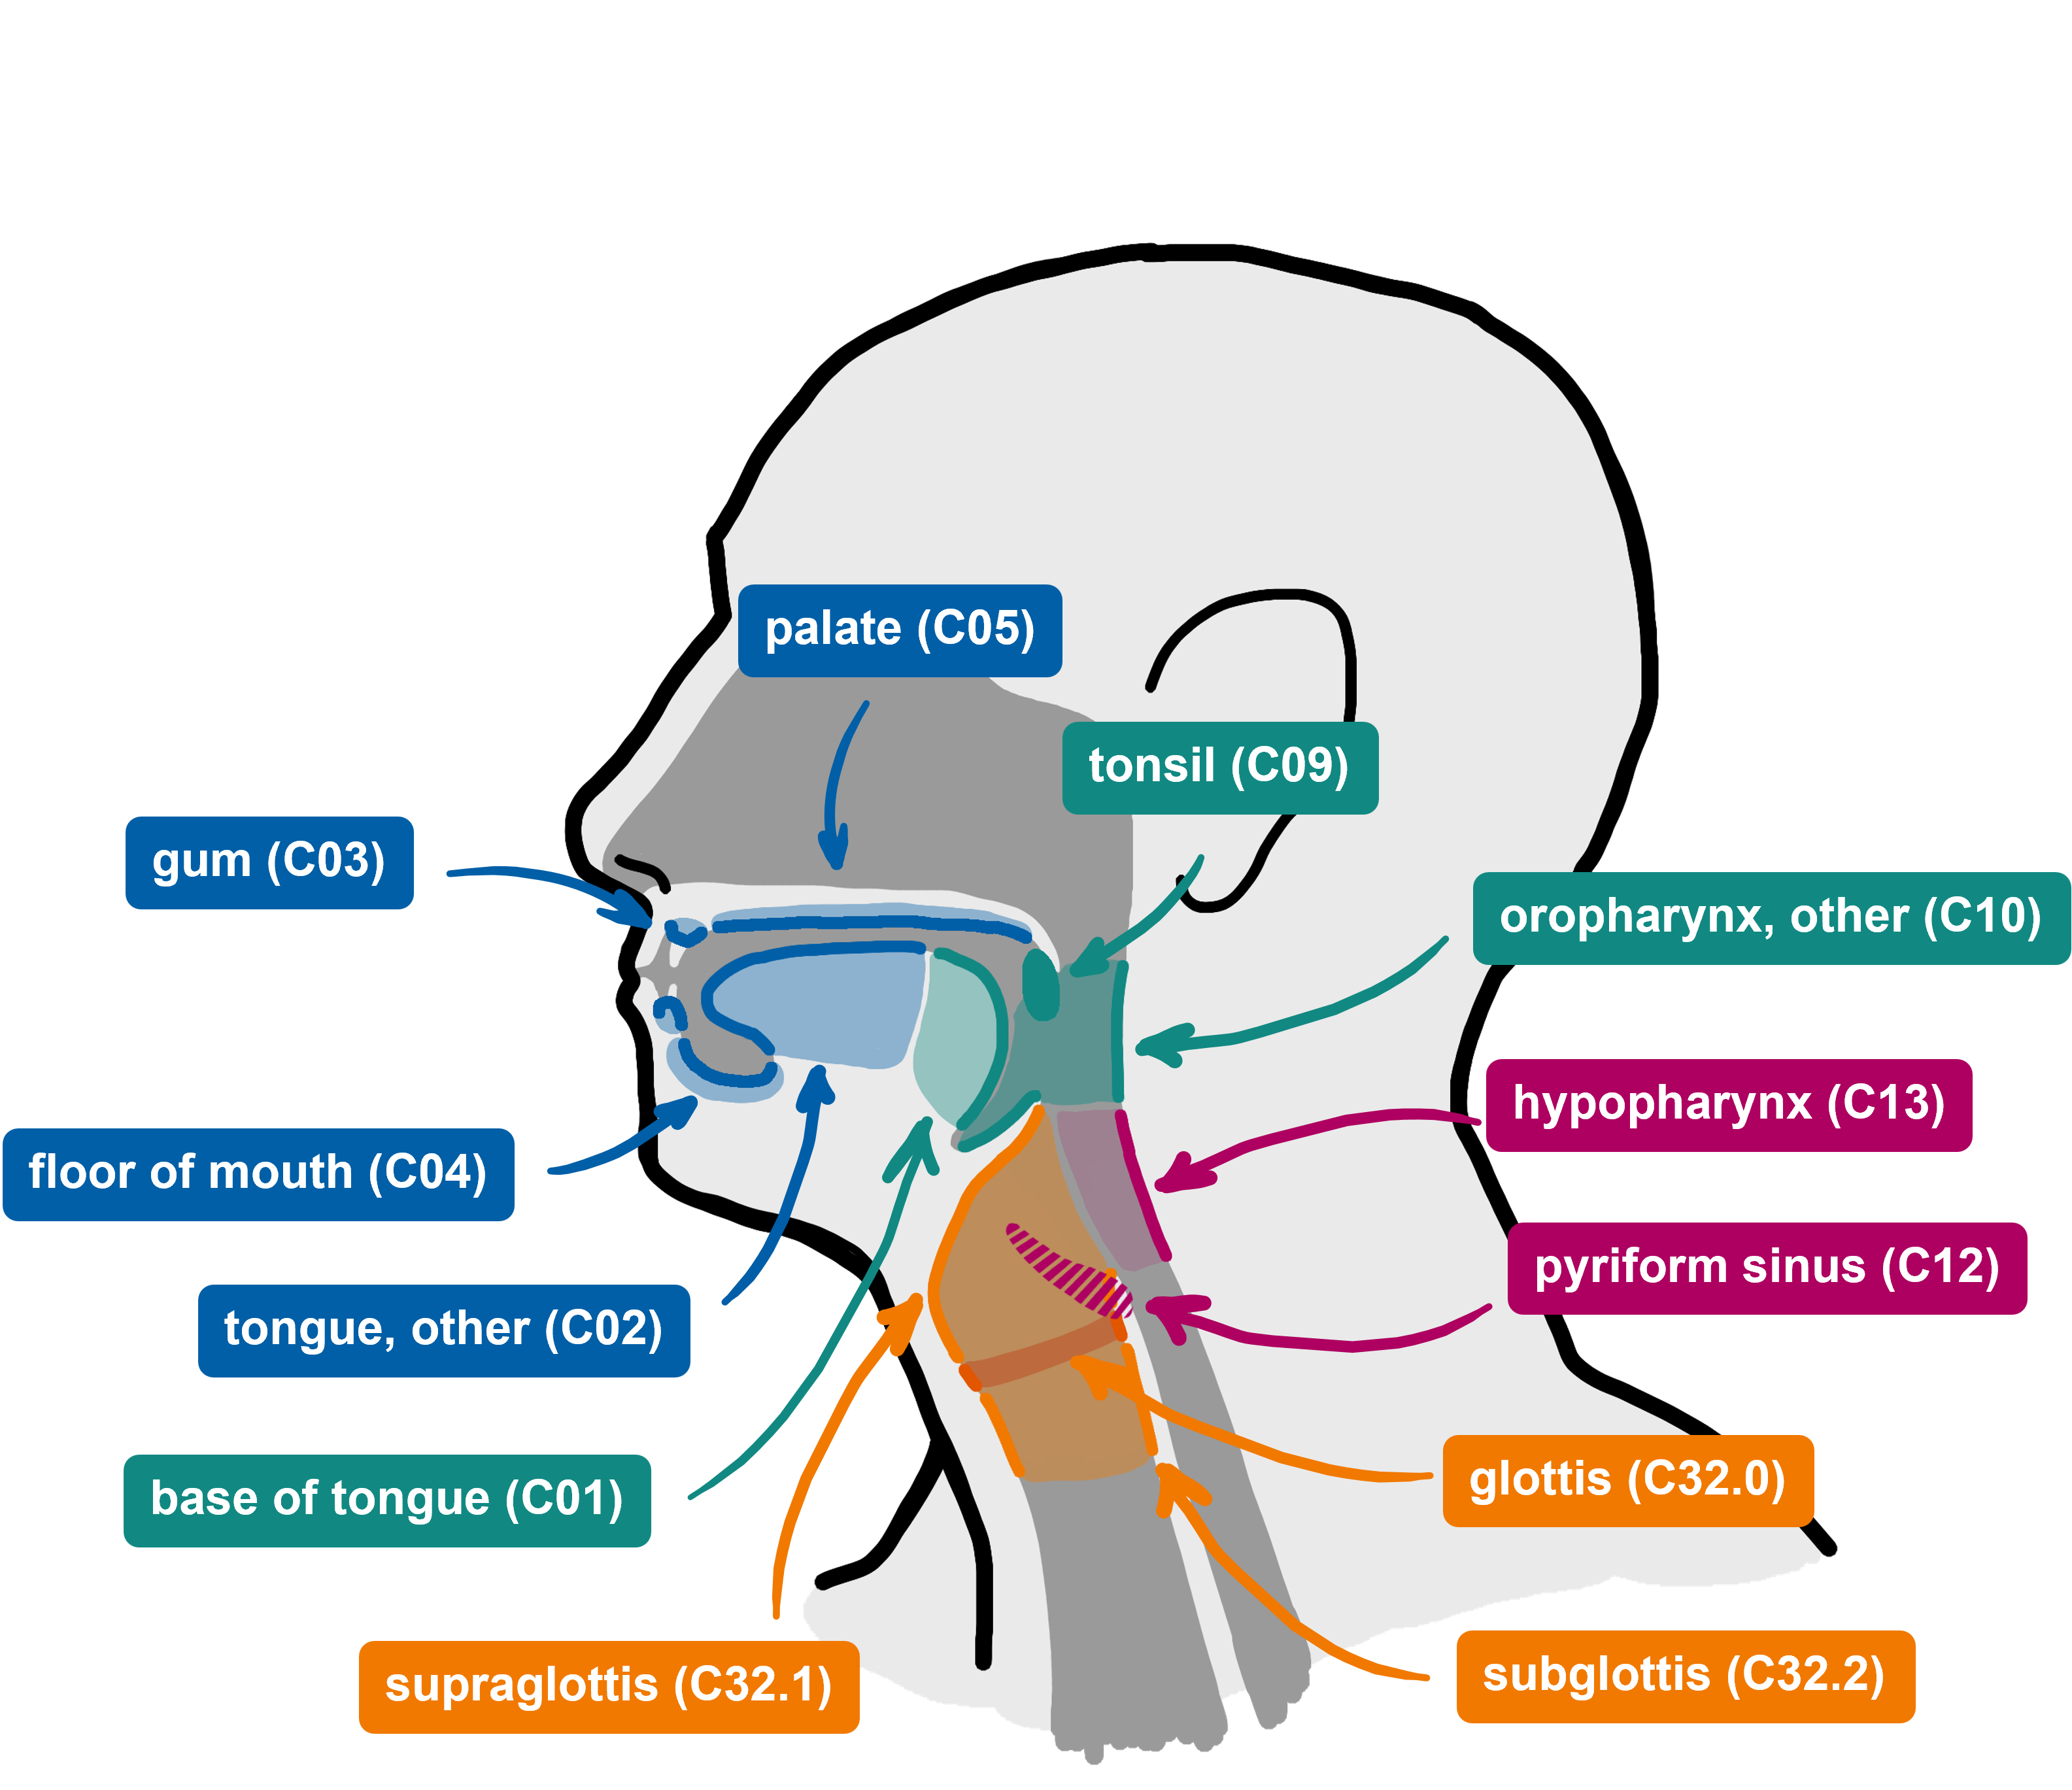
\includegraphics{figures/Subsites.png}

}

\caption{\label{fig-subsites}Anatomical sketch of the tumor subsites and
their corresponding ICD-10 codes. Subsite C06 ``other parts of mouth''
has not been included. Further the The tumor locations are color coded
in the following pattern: blue-oral cavity, green-oropharynx,
red-hypopharynx, orange-larynx.}

\end{figure}%

The prevelance of involvement in LNLs I, II, III, IV and V is shown in
figure~\ref{fig-involvement}. The involvement is stratified per tumor
subsite and t-stage. The figure illustrates the variations in LNL
involvement between subsites within oral cavity (blue), oropharynx
(green), hypopharynx (red) and larynx (orange). The involvement pattern
presents a continuous change over the tumor subsites. Where tumors in
the oral cavity show the most prominent LNL I involvement. As the tumor
location moves towards the oropharynx LNL II involvement increases.
Moving the tumor location further in caudal direction towards the
hypopharynx increases LNL III involvement while LNL I and II involvement
decrease. Larnygeal tumors show the least LNL I involvement.

\begin{figure}

\centering{

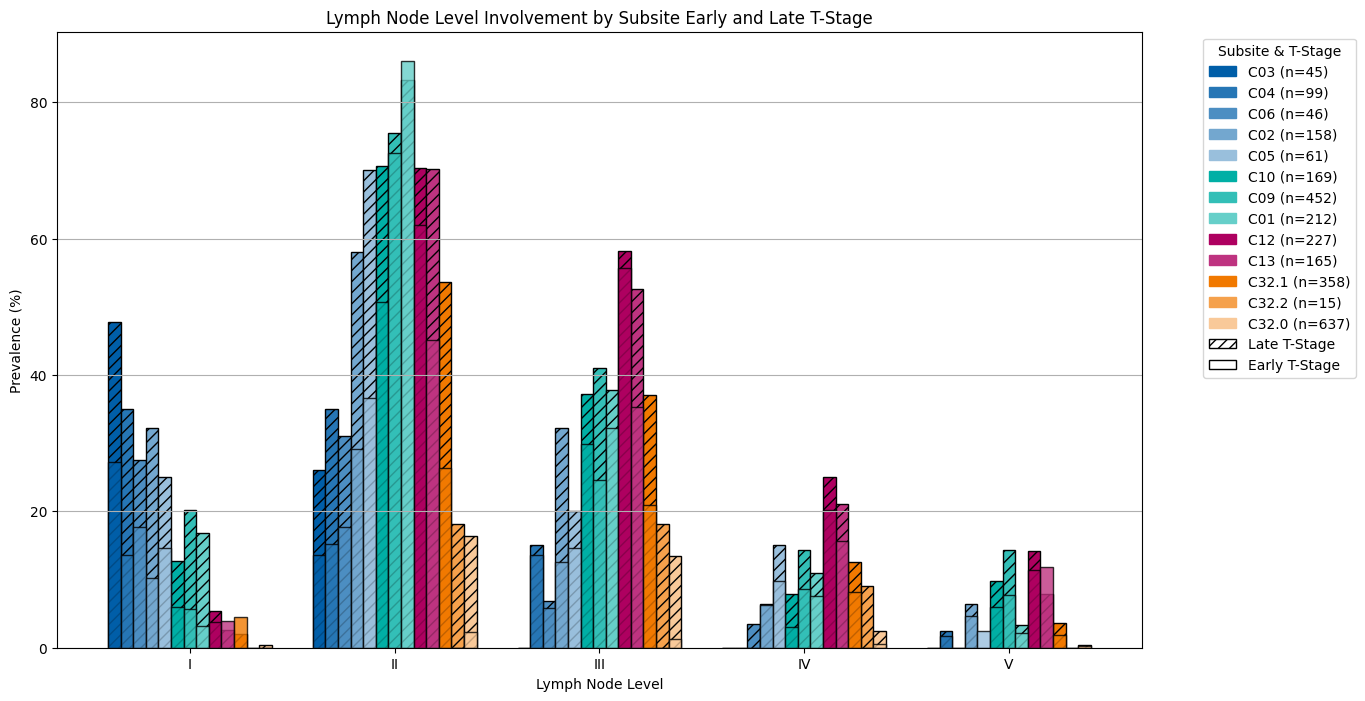
\includegraphics{figures/involvement_I_to_V_all_sites_t_staging.png}

}

\caption{\label{fig-involvement}Prevalence of ipsilateral LNL
involvement stratified by subsite. The subsites are sorted in natural
order to represent the continuously changing LNL involvement. The
different tumo locations are color coded, where oral cavity subsistes
are depicted in blue, larynx in green, hypopharynx in red and larynx in
orange. The patient data is further stratified in early t-stage (0-2)
and late t-stage (3-4). The legend furter specifies the number of
patients in each subsite. For glottis (C32.0) early t-stage only
includes T2.}

\end{figure}%

\section{Unilateral Model for Lymphatic
Progression}\label{sec-unilateral}

In this chapter we will briefly summarize unilateral model for
ipsilateral lymph node involvement introduced in
\citet{ludwig_hidden_2021}, presenting the notation which is then needed
to extend the HMM to a mixture model encompassing multiple tumor
subsites.

The HMM describes each LNL \(v \in 1, 2, ..., V\) by a binary random
variable corresponding to the status of the LNL; healthy (0) or involved
(1). The entire state of a patient with \(V\) LNLs is defined by the
\(V\)-dimensional vector \(\mathbf{X} = [X_1, X_2, ...,X_V]\). In the
HMM, a patient's involvement is modeled over time \(t\). Thus, a
patient's state of lymph node involvement \(\mathbf{X}[t]\) evolves over
discrete time steps \(t\). Let us enumerate all \(2^V\) possible states,
representing all combinations of LNL involvement. In this paper, we
consider ipsilateral LNLs I, II, III, IV and V, which amounts to 32
possible states. The HMM is then specified by a transition matrix
\(\mathbf{A}\):

\begin{equation}\phantomsection\label{eq-transition-matrix}{
\mathbf{A} = \begin{pmatrix} A_{ij} \end{pmatrix} = P \left( \mathbf{X}[t+1] = \boldsymbol{\xi}_j \mid \mathbf{X}[t] = \boldsymbol{\xi}_i \right)
}\end{equation}

whose elements \(A_{ij}\) contain the conditional probabilities that a
state \(\mathbf{X}[t]=\boldsymbol{\xi}_i\) transitions to
\(\mathbf{X}[t+1]=\boldsymbol{\xi}_j\) over one time step. The
transition matrix is specified and parameterised via the graphical model
shown in figure~\ref{fig-graph}. The red arcs in the graph of
figure~\ref{fig-graph} are associated with the probability that the
primary tumor spreads directly to a LNL (parameters \(b_v\)). The blue
arcs describe the spread from an upstream LNL -- given it is already
metastatic -- to a downstream level (parameters
\(t_{v \rightarrow v+1}\)).

\begin{figure}

\centering{

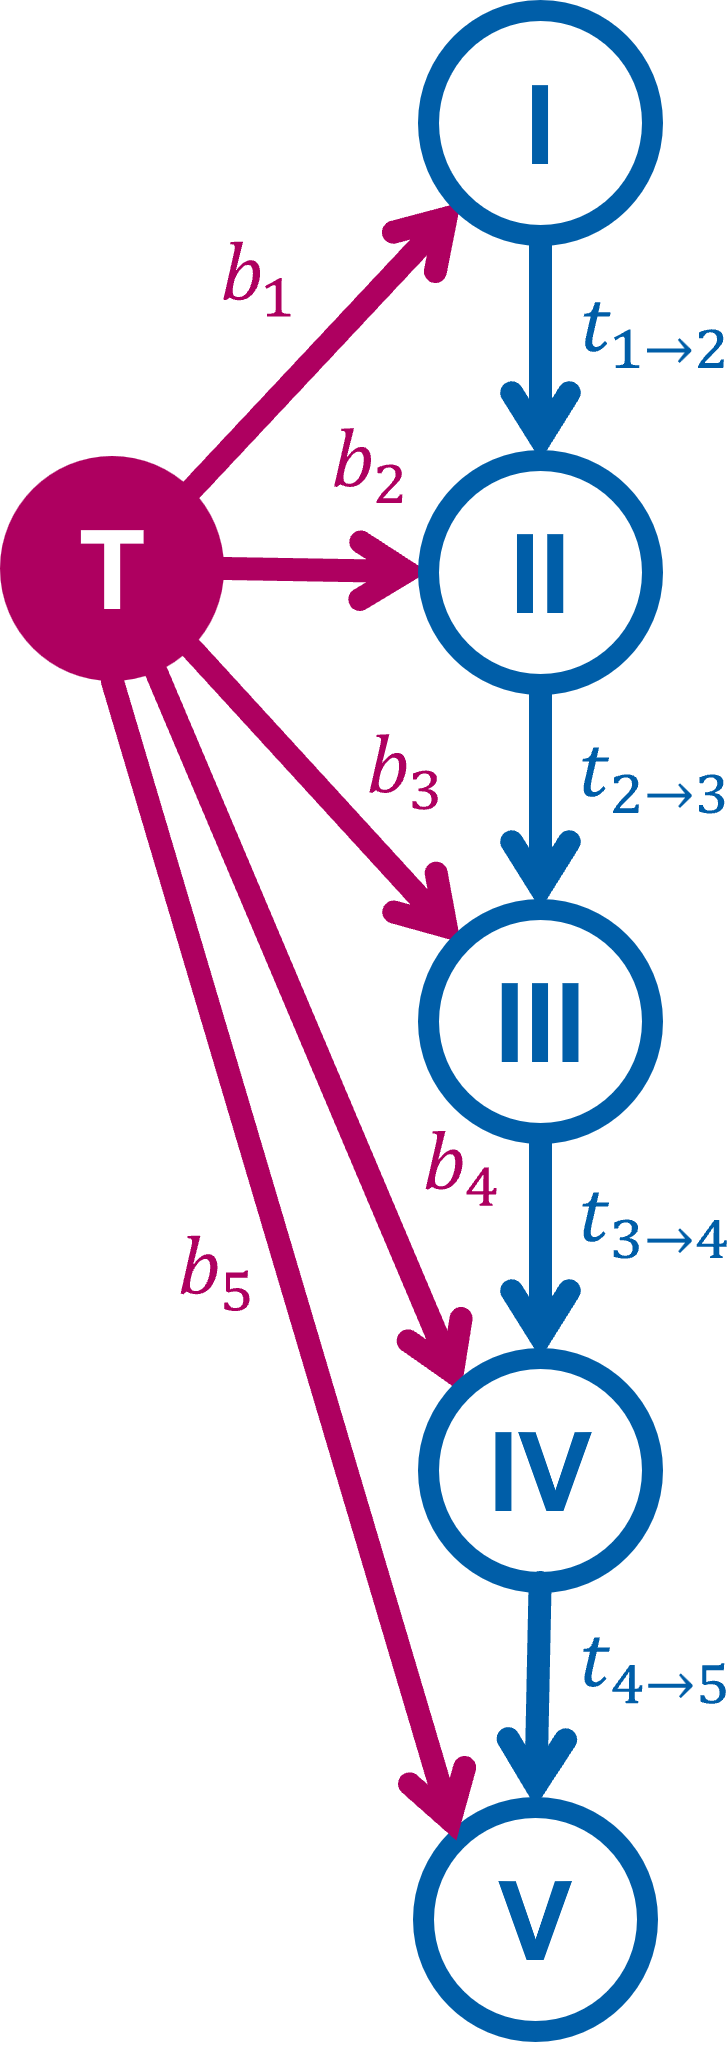
\includegraphics[width=0.2\textwidth,height=\textheight]{figures/Model_5_LNL.png}

}

\caption{\label{fig-graph}Parametrized graphical model of the lymphatic
network considering four LNLs. Blue nodes represent the hidden states of
LNLs \(X_v\), while the red one is the tumor. Arcs represent possible
routes of metastatic spread, associated with a probability.}

\end{figure}%

Now, let \(\boldsymbol{\pi}\) be the \emph{starting distribution}

\begin{equation}\phantomsection\label{eq-starting-distribution}{
\boldsymbol{\pi} = \begin{pmatrix} \pi_i \end{pmatrix} = P \left( \mathbf{X}[0] = \boldsymbol{\xi}_i \right)
}\end{equation}

denoting the probability to start in state \(\boldsymbol{\xi}_i\) at
time step 0. Assuming that every patient started with all LNLs being
healthy, we set \(\pi_i\) to zero for all states except the completly
healthy state
\(\boldsymbol{\xi} = \begin{pmatrix} 0, 0, 0, 0, 0 \end{pmatrix}\),
which has probability one.

Using the quantities introduced so far, the probability
\(P \left( \mathbf{X}[t]=\boldsymbol{\xi}_i \right)\) to be in state
\(\boldsymbol{\xi}_i\) in time step \(t\) can now be conveniently
expressed as a matrix product:

\begin{equation}\phantomsection\label{eq-evolution}{
P \left( \mathbf{X}[t]=\boldsymbol{\xi}_i \right) = \left( \boldsymbol{\pi} \cdot \mathbf{A}^t \right)_i
}\end{equation}

This evolution implicitly marginalizes over all possible paths to arrive
at state \(\boldsymbol{\xi}_i\) after \(t\) time-steps. Additionally, we
must marginalize over the unknown time of diagnosis using a time-prior
\(P_T(t)\) which is defined by a binomial distribution. The t-stage of
the tumor can be included in the model by choosing different
parameterizations of the binomial distribution, considering that a tumor
in late t-stages was diagnosed later than a tumor in early t-stages,
therefore shifting the probability of diagnosis to later time steps.
This finally defines the probability distribution over all states of
lymph node involvement.

\begin{equation}\phantomsection\label{eq-marginalized-evolution}{
P \left( \mathbf{X}=\boldsymbol{\xi}_i \mid \boldsymbol{\theta}, \mathbf{T} \right) = \sum_{t=0}^{t_\text{max}} P_T(t) \left( \boldsymbol{\pi} \cdot \mathbf{A}^t \right)_i
}\end{equation}

where \(\boldsymbol{\theta}=\{ b_v, t_{v \rightarrow v+1} \}\) denotes
the set of all model parameters (7 in our case). Fortunately, the exact
length and shape of this distribution has little impact as previously
shown \citep{ludwig_hidden_2021}. We set \(t_\text{max}=\) 10 and
\(P_\text{early}(t)\) to a binomial distribution with parameter 0.3.
Further details on the HMM can be found in \citet{ludwig_hidden_2021}
and \citet{zora231470}.

With equation~\ref{eq-marginalized-evolution} we can compute the
probability of a patient being in any state \(\xi_i\). To train the
model, we assume that the observed diagnoses in our dataset
\(\mathbf{D}\) directly reflect the underlying hidden states
\(\mathbf{X}\) of the patient. Thus, learning the model parameters
corresponds to maximizing the probability of observing the dataset
\(\mathbf{D}\):

\begin{equation}\phantomsection\label{eq-likelihood-HMM}{
P \left( \mathbf{D} \mid \boldsymbol{\theta} \right) = \prod_k^K P \left( \mathbf{X}_k=\boldsymbol{\xi}_i \mid \boldsymbol{\theta}, T_k \right)
}\end{equation}

In equation~\ref{eq-likelihood-HMM} we compute the likelihood of
observing the diagnosis of each patient \(k\), i.e.~t-stage \(T_k\) and
involvement \(\mathbf{X}_k=\boldsymbol{\xi}_i\).

\subsection{Risk Estimation}\label{risk-estimation}

The goal of the HMM is to predict the risk of occult metastases in LNLs,
given a patient's diagnosis. In this framework this corresponds to
computing the probability of a hidden state
\(\mathbf{X}=\boldsymbol{\xi}_i\) given the observed diagnosis
\(\mathbf{Z}\) and the model parameters \(\boldsymbol{\theta}\). With
Baye's theorem we can compute this probability as follows:

\begin{equation}\phantomsection\label{eq-bayes}{
P(\mathbf{X} =\boldsymbol{\xi}_i \mid \mathbf{Z}, \boldsymbol{\theta}) = \frac{P(\mathbf{Z} \mid \mathbf{X}=\boldsymbol{\xi}_i, \boldsymbol{\theta}) P(\mathbf{X}_k=\boldsymbol{\xi}_i \mid \boldsymbol{\theta})}{P(\mathbf{Z} \mid \boldsymbol{\theta})}
}\end{equation}

where \(P(\mathbf{Z} \mid \boldsymbol{\theta})\) is the marginal
likelihood of the data, which can be computed by summing over all
possible hidden states \(\boldsymbol{\xi}_i\):

\begin{equation}\phantomsection\label{eq-marginal-likelihood}{
P(\mathbf{Z} \mid \boldsymbol{\theta}) = \sum_{\boldsymbol{\xi}_i} P(\mathbf{Z} \mid \boldsymbol{\xi}_i, \boldsymbol{\theta}) P(\boldsymbol{\xi}_i \mid \boldsymbol{\theta})
}\end{equation}

With this we can compute the probability for each hidden state and
subsequently we can compute the probability for each LNL \(v\) to be
involved given the diagnosis \(\mathbf{Z}\) and the model parameters
\(\boldsymbol{\theta}\) by summing over all possible hidden states
\(\boldsymbol{\xi}_{i,v}\) where the LNL \(v\) is involved:

\begin{equation}\phantomsection\label{eq-risk}{
P(X_v=1 \mid \mathbf{Z}, \boldsymbol{\theta}) = \sum_{\boldsymbol{\xi}_{i,v}} P(\mathbf{X} =\boldsymbol{\xi}_i \mid \mathbf{Z}, \boldsymbol{\theta})
}\end{equation}

As opposed to the model training, we do not assume anymore that the
diagnoses correspond to the hidden states. Instead, we consider the
sensitivity and specificity of the diagnostic modalities used to
determine the involvement of LNLs. Enabling the uncertainty originating
from diagnostic modalities to be considered in the model. Here we chose
the sensitivity of 0.81 for clinical modalities corresponding to the
literature value for imaging modalities \citep{de_bondt_detection_2007}
and specificity of 1.0, indicating that all positively diagnosed LNLs
are indeed involved.

\section{Mixture Model for Lymphatic Spread}\label{sec-mixture}

Primary tumors at different subsites exhibit distinct lymphatic spread
patterns. This presents a challenge when attempting to generalize
predictive models across subsites. One approach, as introduced in
\citep{ludwig_dynamic_2021}, uses a Hidden Markov Model (HMM) trained
specifically for oropharyngeal cancer. However, extending this model to
other subsites would either require generalizing over several subsites
or training a separate model for each. The former approach sacrifices
precision, particularly for subsites with fewer patients, while the
latter approach becomes computationally intensive and introduces large
uncertainties for subsites with limited patient data, such as C04 (Floor
of mouth) or C05 (Palate).

To address these challenges and exploit the anatomical similarities
between nearby subsites, we introduce a mixture model that combines data
from all subsites into a single model. This model accounts for
anatomical proximities, thereby improving predictive power while
maintaining computational efficiency.

\subsection{Mixture Model Formulation}\label{mixture-model-formulation}

The mixture model assumes that the data is generated by a set of \(M\)
different lymphatic spread models. Each patient \(k\), with their
primary tumor in subsite \(s \in (1, 2, \ldots, S)\), is assumed to be
generated by one specific model \(m \in (1, 2, \ldots, M)\) from this
set of \(M\) models with probability \(\pi_m^s\). These so-called
\emph{mixing parameters}
\(\boldsymbol{\pi}^s = \{\pi_1^s, \pi_2^s, \dots, \pi_M^s\}\) must
satisfy the condition

\[
\sum_{m}^M \pi_m^s = 1, \quad \forall s
\]

If we could record the componet \(m\) from which a patient \(k\) was
drawn from, we could store this information in a binary latent vector
\(\boldsymbol{\epsilon}_k\). The vector \(\boldsymbol{\epsilon}_k\) has
length \(M\), with exactly the \(m\)-th element set to 1, indicating
which model generated the patient's data, and all other elements set to
0. Thus, for patient \(k\), the latent variable
\(\boldsymbol{\epsilon}_k\) can be interpreted as a categorical
indicator variable that encodes the assignment to one of the \(M\)
lymphatic spread models. Typically in mixture models, this so-called
\emph{latent variable} is unknown. However, it can be inferred and is
useful for inferring the models' parameters.

The joint probability of the observed data \(\mathbf{D}\) (i.e., patient
data) and the latent variables \(\boldsymbol{\epsilon}\) - sometimes
called the \emph{complete data likelihood} - is given by:

\begin{equation}\phantomsection\label{eq-complete-likelihood}{
P(\mathbf{D}, \boldsymbol{\epsilon} \mid \boldsymbol{\theta}, \boldsymbol{\pi}) = \prod_{k}^{K} \prod_{m}^{M} \left[ \pi_m^{s_k} P(\mathbf{D}_k \mid \boldsymbol{\theta}_m) \right]^{\epsilon_{k}^m}
}\end{equation}

Here:

\begin{itemize}
\tightlist
\item
  \(\pi_m^{s_k}\) is the mixing coefficient for subsite \(s_k\) (where
  patient \(k\) has their tumor) and model \(m\),
\item
  \(P(\mathbf{D}_k \mid \boldsymbol{\theta}_m)\) is the likelihood of
  patient \(k\)'s diagnosis, i.e.~The involvement state
  \(\mathbf{X}_k = \boldsymbol{\xi}_i\) and t-stage \(T_k\), given that
  it was generated by model \(m\),
\item
  \(\boldsymbol{\theta}_m\) represents the parameters of model \(m\),
\item
  \(\epsilon_{k}^m\) is the latent variable that indicates patient \(k\)
  was generated by model \(m\).
\end{itemize}

In contrast, the \emph{incomplete data likelihood} marginalizes over all
possible latent assignments to reflect the uncertainty about which model
generated each patient's data:

\begin{equation}\phantomsection\label{eq-incomplete-likelihood}{
P(\mathbf{D}, \mid \boldsymbol{\theta}, \boldsymbol{\pi}) = \prod_{k}^{K} \sum_{m}^{M} \pi_m^{s_k} P(\mathbf{D}_k \mid \boldsymbol{\theta}_m)
}\end{equation}

Ultimately, we want to find the parameters which maximize this
likelihood function for the given data.

Note the summation inside the product. This structure of mixture models
makes naive inference difficult, because the logarithm of this quantity
is expensive to compute and not easy to differentiate. Thus, inferring
the latent assignment is helpful, because the complete data
(log-)likelihood (equation~\ref{eq-complete-likelihood}) does not suffer
from this shortcoming.

To infer the latent assignment \(\boldsymbol{\epsilon}_k\), we start
with its distribution, given the observed data and model parameters:

\begin{equation}\phantomsection\label{eq-responsibilities}{
\gamma(\epsilon_k^m) := \mathbb{E}[\epsilon_k^m] = \frac{\pi_m^{s_k} P \left( \mathbf{D}_k \mid \boldsymbol{\theta}_m \right)}{\sum_{j \leq M} \pi_j^{s_k} P \left( \mathbf{D}_k \mid \boldsymbol{\theta}_j \right)}
}\end{equation}

This expectation value - often called the \emph{responsibility} -
describes the probability that patient \(k\) was generated by model
\(m\). It can be used to compute the expected complete data likelihood:

\begin{equation}\phantomsection\label{eq-expected-complete-likelihood}{
\mathbb{E}_{\boldsymbol{\epsilon}} \left[ P \left( \mathbf{D}, \boldsymbol{\epsilon} \mid \boldsymbol{\theta}, \boldsymbol{\pi} \right) \right] = \prod_{k=1}^K \prod_{m=1}^M \left[ \pi_m^{s_k} P \left( \mathbf{D}_k \mid \boldsymbol{\theta}_m \right) \right]^{\gamma(\epsilon_k^m)}
}\end{equation}

This expected complete data likelihood has the same tractable form as
equation~\ref{eq-complete-likelihood} and thus allows us to infer both
the mixing coefficients \(\boldsymbol{\pi}\) as well as each component
model's parameters \(\boldsymbol{\theta}_m\) using straightformward
inference. Also, these two sets of parameters are the only ones used for
the later risk prediction. The responsiblities \(\gamma(\epsilon_k^m)\)
are only used during inference.

In figure~\ref{fig-model-simple} the mixture coefficients are
illustrated. Subsites with different spread patterns, such as Gum (C03)
and Base of tongue (C01), are expected to get different model
assignments. Nonetheless, the latent variables for two patients with the
same diagnosis, i.e.~same involvement \(\boldsymbol{\xi}\) and and
t-stage \(T\), but different subsites are the same.

\begin{figure}

\centering{

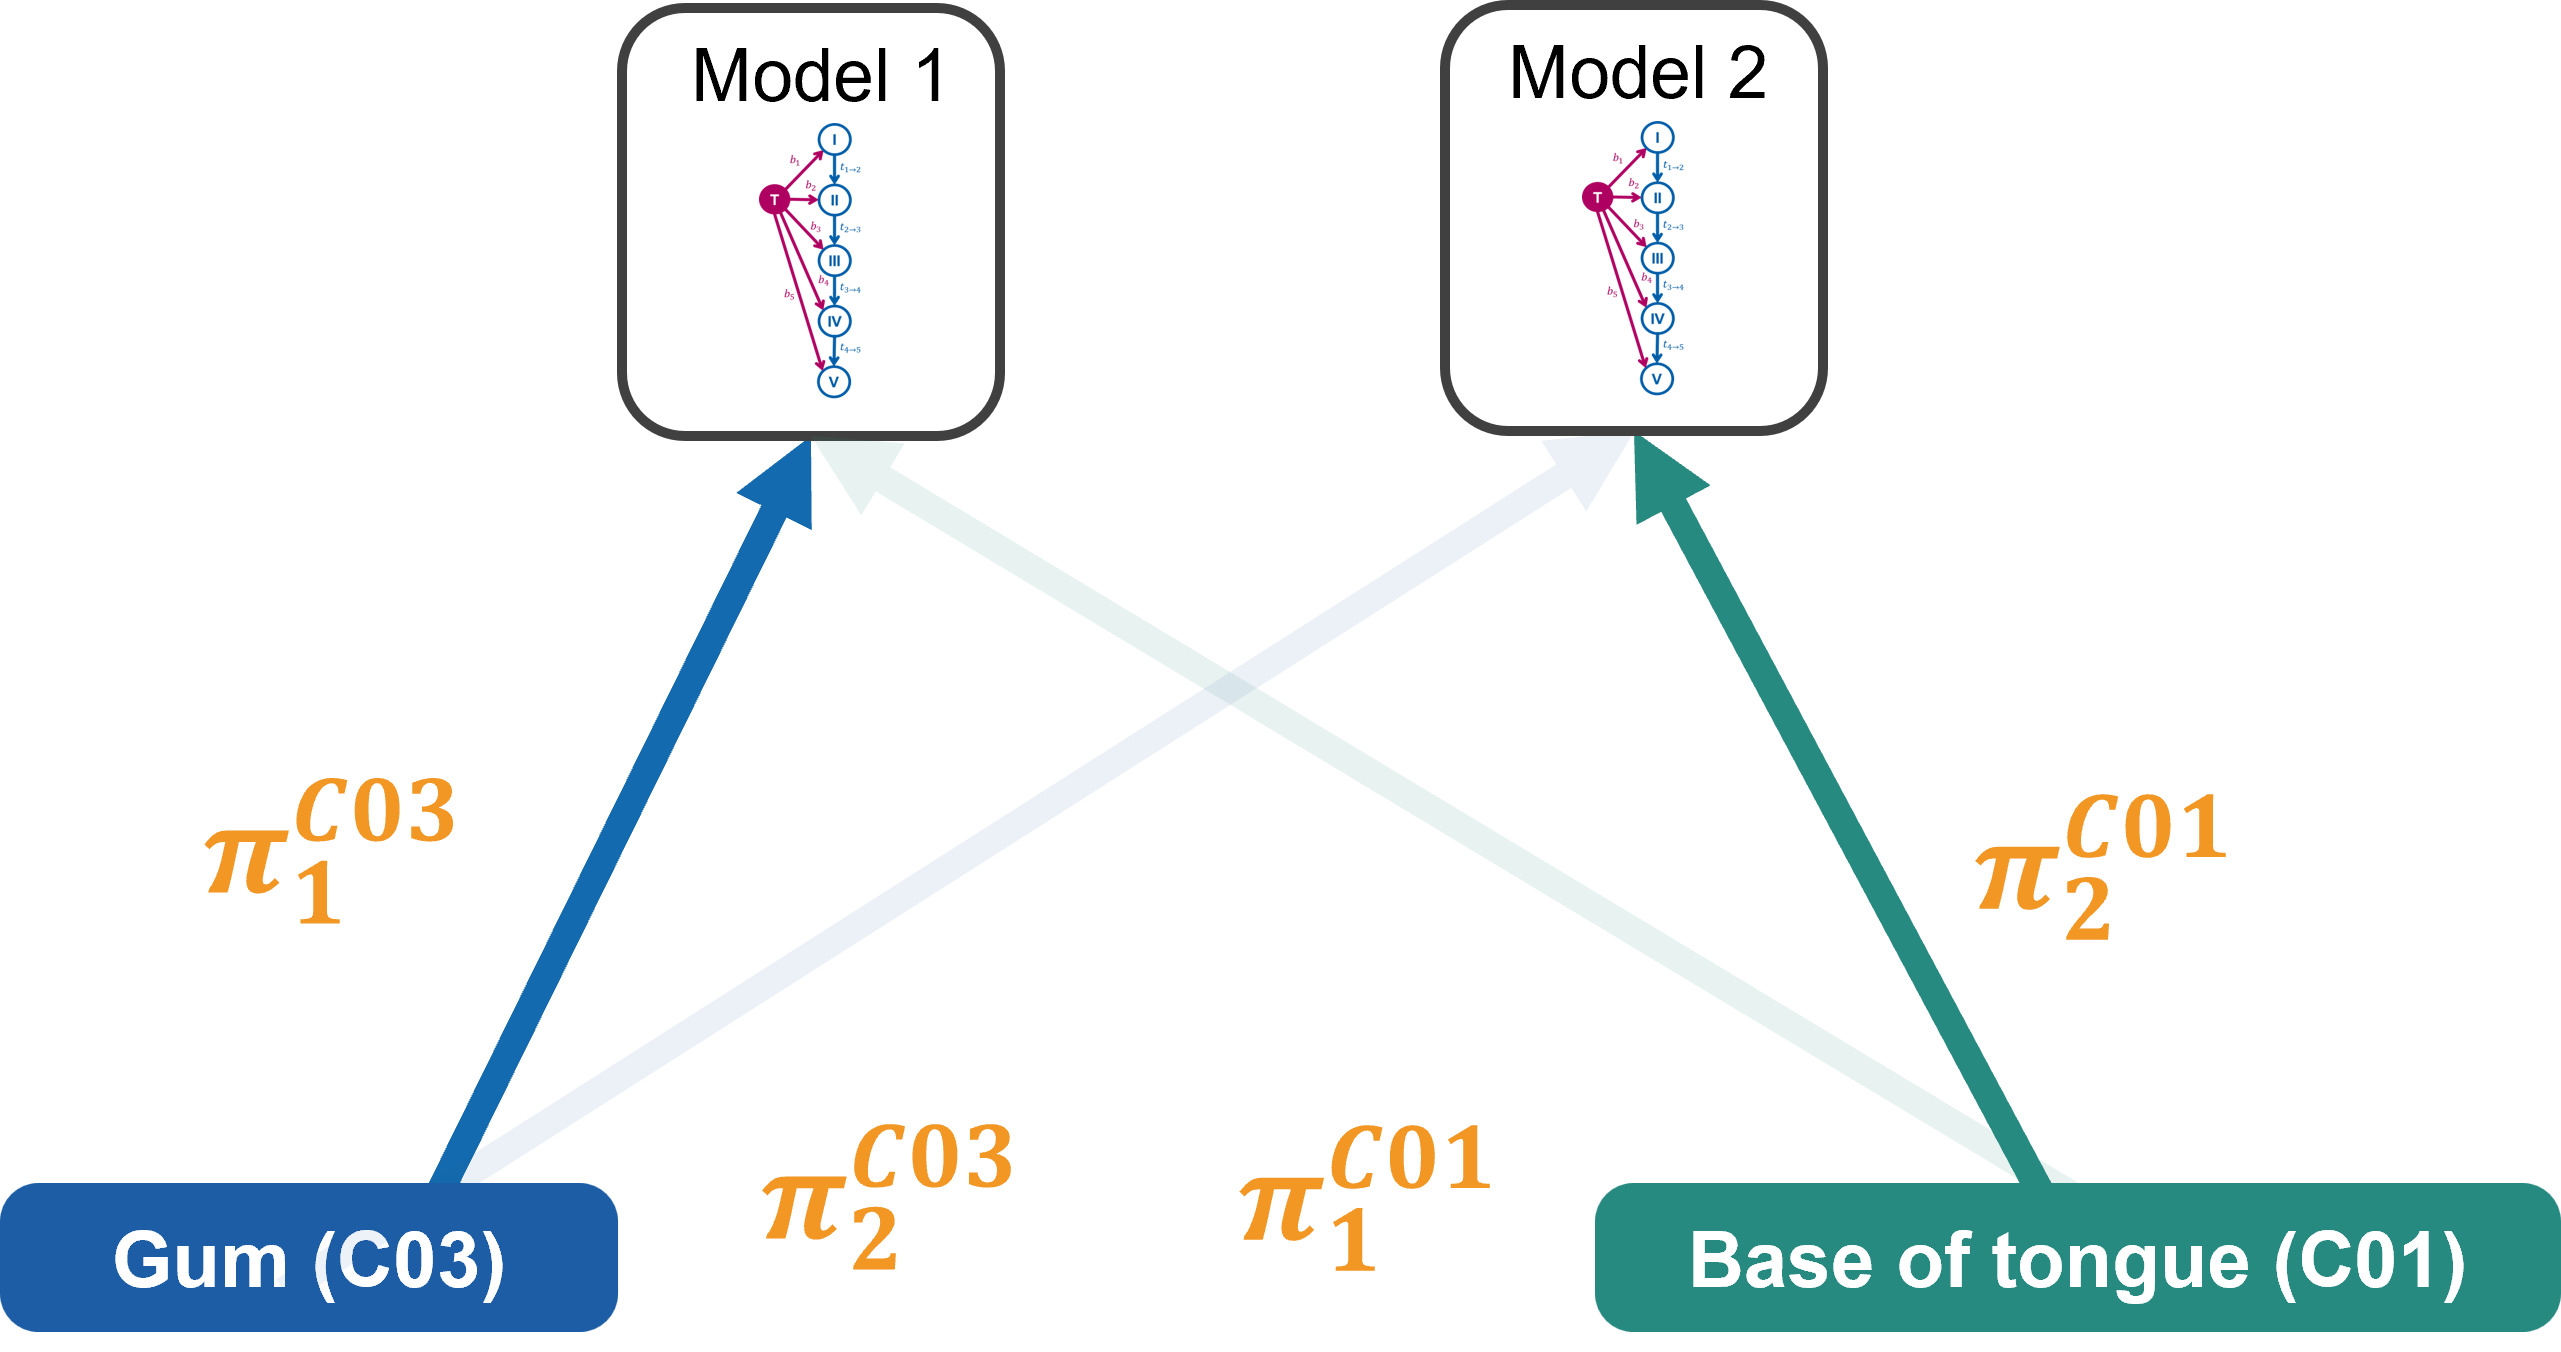
\includegraphics{figures/mixture_model_simplified.png}

}

\caption{\label{fig-model-simple}Illustration of mixture parameter
assignment. Since Gum and Base of tongue express different spread
patterns, the two models are expected to have different model
assignments. The arrow visibility represents the value of the mixture
parameter \(\pi\), where the more visible the arrow, the larger the
value for \(\pi\)}

\end{figure}%

It is important to note that this mixture model algorithm diverges from
the conventional formulation of mixture models as introduced in
\citet{bishop_pattern_2006}. In Bishop's work, the mixture model is
defined with a single set of mixture parameters \(\boldsymbol{\pi}\),
implying that all data points are generated from the same mixture of
models. In our approach, however, we categorize the data points
(patients) into distinct cohorts (subsites), with each subsite
characterized by its own set of mixture parameters. Consequently, we
construct \(S\) separate mixture models, each possessing different
mixture parameters while all models share the same underlying
probability distributions, specifically the varying lymphatic spread
models.

\subsection{Expectation-Maximization (EM)
Algorithm}\label{expectation-maximization-em-algorithm}

To find the mixing coefficients \(\boldsymbol{\pi}\) and all models'
parameters \(\boldsymbol{\theta}_m\) that maximize
equation~\ref{eq-incomplete-likelihood}, we follow an iterative approach
called \emph{expectation-maximization} or \emph{EM-algorithm}. With
arbitrarily initialized starting parameters, we alternate between the
following two steps:

\begin{enumerate}
\def\labelenumi{\arabic{enumi}.}
\tightlist
\item
  In the \textbf{E}xpectation step, we compute the responsibilities
  \(\gamma(\epsilon_k^m)\), which represent the probabilities of a
  patient \(k\) originating from one of the models \(m\), given the
  current estimates of \(\boldsymbol{\theta}\) and \(\boldsymbol{\pi}\),
  as given in equation~\ref{eq-responsibilities}.
\item
  During the \textbf{M}aximization step, we find a new set of parameters
  that maximize the new expected complete data likelihood
  (equation~\ref{eq-expected-complete-likelihood}). For the mixture
  coefficients, we can even find an analytic solution to the new
  maximum: \[
  \pi_m^s = \frac{1}{|K_s|} \sum_{k \in K_s} \gamma(\epsilon_k^m)
  \] where we sum over the set of all patients \(K_s\) with their tumor
  in subsite \(s\).\\
  The models' new parameters are found by numerically maximizing the
  respective likelihood, weighted by the responsibilities:
  \begin{equation}\phantomsection\label{eq-maximization-step}{
  \ln P(\mathbf{D}, \boldsymbol{\epsilon} \mid \boldsymbol{\theta}_m) = \sum_k^K \gamma(\epsilon^m_{k}) \big[ \ln \pi_m^{s_k} + \ln P \left( \mathbf{D}_k \mid \boldsymbol{\theta}_m \right) \big]
  }\end{equation}
\end{enumerate}

By iterating these steps, the EM algorithm is guaranteed to converge to
a (local) maximum of the incomplete data likelihood
(equation~\ref{eq-incomplete-likelihood}).

\subsection{Uncertainty estimation}\label{sec-uncert}

To estimate the uncertainty associated with both the model parameters
and the resulting risk estimates, we employ a bootstrapping approach.
Although more comprehensive sampling methods exist for the EM
algorithm---such as the imputation-posterior (IP) algorithm, which
samples from both model parameters and latent variables---we opt for a
computationally more efficient alternative that still yields multiple
estimates of all parameters.

Our resampling procedure involves the following steps:

\begin{enumerate}
\def\labelenumi{\arabic{enumi}.}
\item
  Resample the observed data with replacement, maintaining the original
  number of samples per ICD code.
\item
  Fit the model to each resampled dataset.
\item
  Extract the model parameters and risk estimates from each fitted
  model.
\end{enumerate}

This method enables a straightforward uncertainty analysis while
avoiding the computational cost of more intensive sampling techniques.

\section{Model Training Evaluation}\label{sec-model_train}

In the following sections we will analyze the model training for three
components first, considering Oral Cavity, Oropharynx and Hypopharynx
data. Then we extend the model to four components, additionally
including Larynx data. Both models will include LNLs I, II, III, IV and
V. LNLs VI and VII are omitted for simplicity and since the prevalence
for these LNLs never exceeds 11\% (figure~\ref{fig-involvement}),
meaning that the risk of involvement is low in most cases.

\subsection{Three Component Mixture Model}\label{sec-3comp}

We first evualuate the methodology for a mixture model with M = 3
components. We include the ICD codes as subsites for oral cavity,
hypopharynx and oropharynx. In figure~\ref{fig-convergence} the
convergence of the negative log-likelihood and change in model
parameters is depicted. After a random inizialization, the algorithm
rapidly converges. The algorithm was stopped when the difference of
log-likelihood between two iterations was below 0.01.

\begin{figure}

\centering{

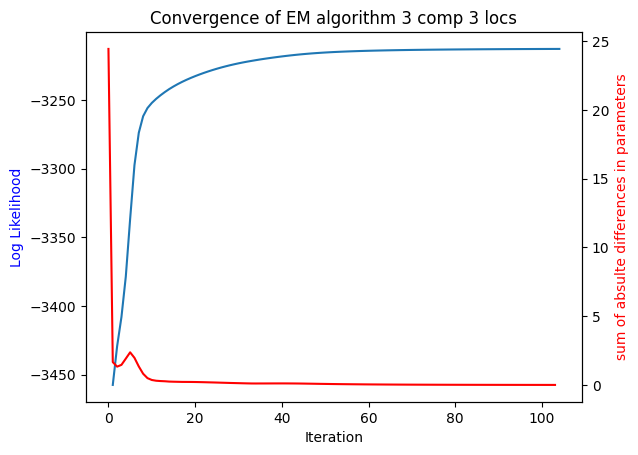
\includegraphics{figures/Convergence_3_comp.png}

}

\caption{\label{fig-convergence}The y-axis on the left shows the
negative likelihood convergence depicted in the blue line. The y-axis on
the right shows the sum of absulte difference between all model
parameters showing that the parameter values stabilize rapidly as well.}

\end{figure}%

In figure~\ref{fig-3_simplex}, we visualize the resulting mixture
coefficients \(\boldsymbol{\pi}\) using a spatial representation, where
the vertices of the triangle correspond to the three components. In
figure~\ref{fig-3-matrix}, these mixture coefficients are presented in
matrix form, with the y-axis representing the ICD codes, showing how the
mixture components in each row add up to 1.

The spatial plot in figure~\ref{fig-3_simplex} illustrates how the model
assigns the three components to different tumor subsites. Component 0,
located at the bottom right of the triangle, primarily characterizes
hypopharyngeal subsites. Both hypopharyngeal subsites, piriform sinus
(C12) and hypopharynx (C13), are strongly assigned to this component.
Similarly, component 1, located at the bottom left, characterizes oral
cavity subsites. For instance, the gum (C03), which has the highest LNL
I involvement is fully assigned to this subsite. As subsites
anatomically approach the oropharynx, their mixture coefficients for the
oropharynx-like component, at the top of the triangle, increase. This is
evident in the subsites C02 (tongue) and C05 (palate), which display a
higher proportion of oropharyngeal influence in their mixture. These
results conform well with the involvement patterns observed in the data
in figure figure~\ref{fig-involvement}. The base of tongue subsite
(C01), which exhibits the highest involvement of LNL II, is fully
assigned to oropharynx-like component. Similarly, subsite C10, which
includes several oropharyngeal regions, is assigned roughly 50\% to the
oropharynx-like component, with the remaining mixture distributed across
the other two components, representing its large variation in spread
patterns.

\begin{figure}

\begin{minipage}{0.71\linewidth}

\begin{figure}[H]

\centering{

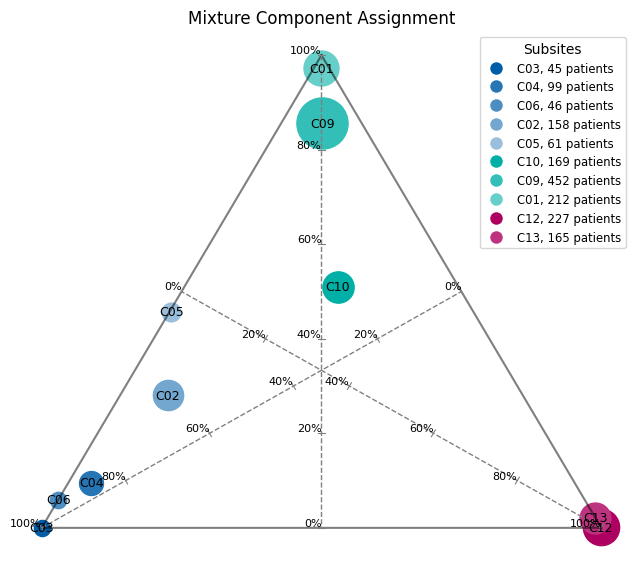
\includegraphics{figures/mixture_components_3_simplex.png}

}

\caption{\label{fig-3_simplex}Assignment of each subsite to each of the
three components. The closer a subsite is to a vertex, the more it is
assigned to the corresponding component, with component 0 on the bottom
right, 1 on the bottom left and 2 on the top. The size of the marker
(area) corresponds to the number of patients in each subsite.}

\end{figure}%

\end{minipage}%
%
\begin{minipage}{0.29\linewidth}

\begin{figure}[H]

\centering{

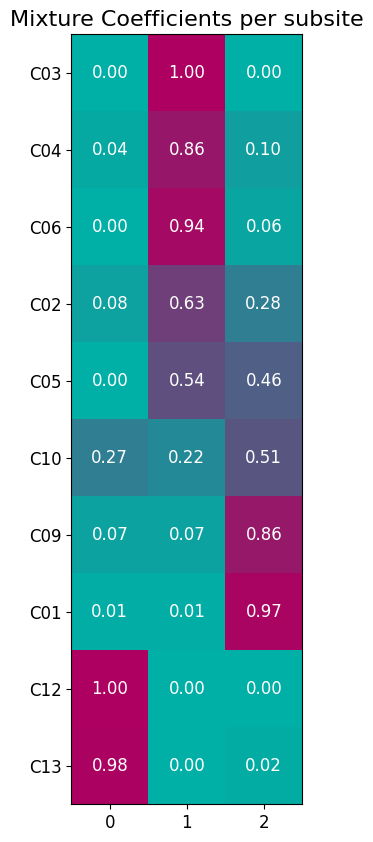
\includegraphics{figures/mixture_components_3.png}

}

\caption{\label{fig-3-matrix}Matrix representation of component
assignment. Each row of the matrix corresponds to each ICD code. The
collums represent the three different components}

\end{figure}%

\end{minipage}%

\end{figure}%

To evaluate the uncertainty in the model parameters, the bootstrapping
approach introduced in section~\ref{sec-uncert} has been applied.
Specifically, we generated 200 bootstrap samples by resampling the
observed data with replacement, maintaining the original number of
samples per ICD code. For each bootstrap sample, the mixture model was
re-fitted, and the resulting parameters were recorded. This process
yielded a distribution of parameter estimates, allowing us to compute
confidence intervals and assess the variability in the model's
predictions.

The results of the bootstrapping analysis are shown in
figure~\ref{fig-simplex_uncert} and
figure~\ref{fig-3_comp_scatter_uncert}. The figure illustrates the
variability in the mixture coefficients \(\boldsymbol{\pi}\) for each
subsite in the same representation as figure~\ref{fig-3_simplex}. The
figure shows that the uncertainties match the continuity of the spread
patterns. The base of tongue (C01) has most of its uncertainty along in
between the oropharynx component and the hypopharynx component.
Similarly, the hypopharynx subsite (C13) mostly presents uncertainty
between these two components. The more general oropharnyx subsite (C10)
shows more uncertainty in each components direction, due to its mixed
spread pattern. The subsite for other pars of mouth (C03) however, only
has uncertainty along the axis connecting the oropharyngeal component
and the oral cavity componen, therefore never mixing with the
hypopharynx-like component on the right. In figure
figure~\ref{fig-3_comp_scatter_uncert} the asymmetry of the uncertainty
is better depicted. E.g. the base of tongue (C01) subsite and the
hypopharynx (C13) subsite have strongly asymmetric uncertainties.
Further, the plot better characterizes the uncertainty in the palate
subsite (C05), where the mixture and uncertainty is mainly in the
oropharynx-like and the oral cavity-like components if we center the
uncertainty around the optimal values instead of the mean values as it
is depicted in figure~\ref{fig-simplex_uncert}.

\begin{figure}

\centering{

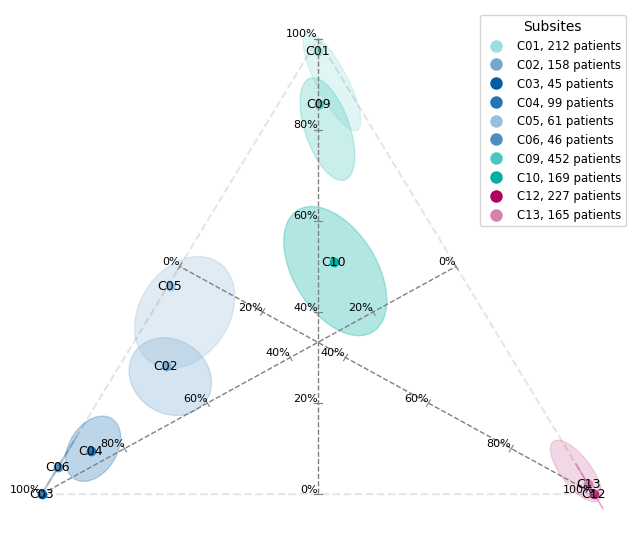
\includegraphics{figures/mixture_coefficients_uncert_simplex.png}

}

\caption{\label{fig-simplex_uncert}Variability in mixture coefficients
\(\boldsymbol{\pi}\) across bootstrap samples for each subsite. Where
the dots represent the optimal values and the ellipses represent the
68\% percentile centered around the mean value. The 68\% percentile are
computed assuming a 2D-gaussian distribution. However, with the bounds
of 0 and 1 the sampled mixture coefficients do not exactly follow a
gaussian distribution.}

\end{figure}%

\begin{figure}

\centering{

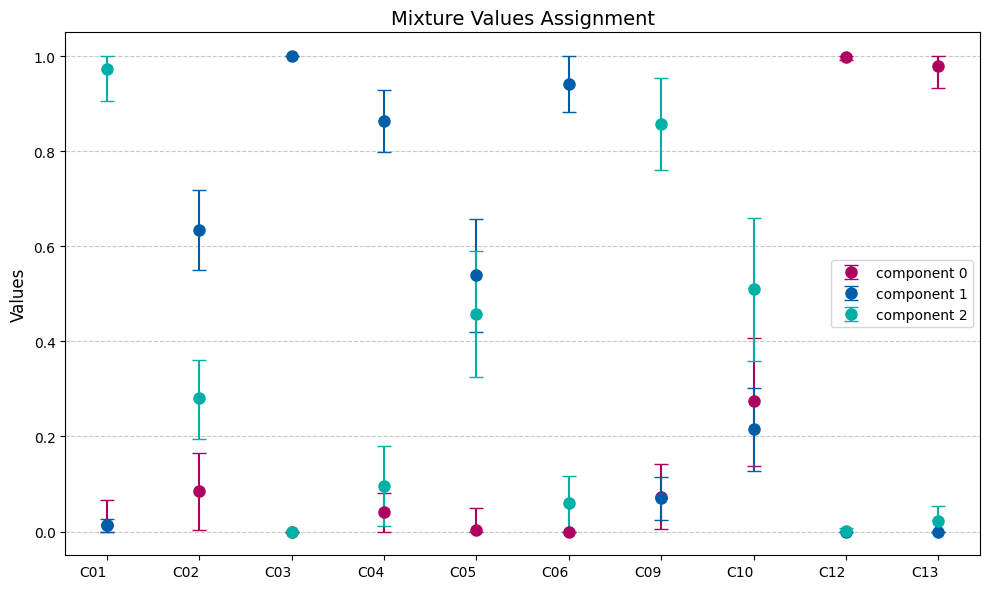
\includegraphics{figures/3_comp_mixture_coefficients_uncert_scatter.png}

}

\caption{\label{fig-3_comp_scatter_uncert}Variability in mixture
coefficients \(\boldsymbol{\pi}\) across bootstrap samples for each
subsite. The dots represent the optimal values. The bars include 68\% of
all sample values centered around the optimal values.}

\end{figure}%

Additionally, the bootstrapping approach enables us to quantify the
uncertainty in the model predictions for each subsite and LNL. To
benchmark the model we analyze the predicted and observed prevalences
for LNLs I, II, III, IV, and V. These predictions are stratified by
tumor subsite and t-stage, providing a comprehensive view of the model's
performance and its associated uncertainty.

In figure~\ref{fig-oral_cavity} we present the predictions for the oral
cavity subsites C03 and C05. Here we can clearly see in figure
figure~\ref{fig-oral_cavity_C03_early} and
figure~\ref{fig-oral_cavity_C03_late} that the difference in prevalence
is substantial, even though both subsites are grouped in the same tumor
location. The model predicts a higher prevalence for LNL II in subsite
C05 (palate) compared to subsite C03 (gum). This is consistent with the
observed data, where the prevalence of LNL II involvement is higher for
the palate than for the gum. However, the model only predicts a slightly
higher prevalence for LNL I in subsite C03 compared to subsite C05. This
is not consistent with the observed data, where the prevalence of LNL I
involvement is significantly higher for the gum than for the palate.
Thus, showing a limitation in the model to properly split these
different involvements. In late t-stages, depicted in figure
figure~\ref{fig-oral_cavity_C03_late} and
figure~\ref{fig-oral_cavity_C05_late}, the model predicts a higher
prevalence for LNL II in subsite C05 compared to the early t-stage, but
not fully capturing the increase in prevalence. For subsite C03 the LNL
II involvement is predicted to increase as well, capturing the increase
in prevalence. However, for LNL I, while capturing the increase in
prevalence, it does not optimally predict the prevalence, similarly to
the early t-stage. For LNLs III, IV and V, the model consistently
predicts the low prevalences observed in the data for both subsites.

\begin{figure}

\begin{minipage}{\linewidth}

\centering{

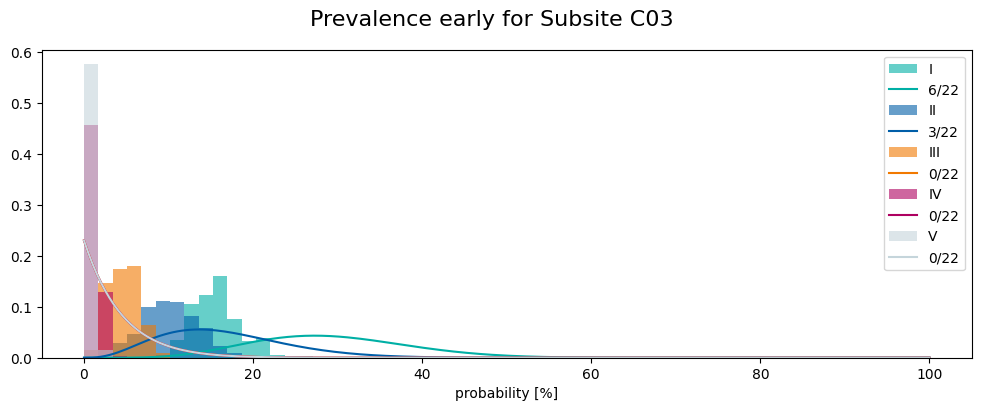
\includegraphics{figures/3_predicted_prevalence_C03_early.png}

}

\subcaption{\label{fig-oral_cavity_C03_early}}

\end{minipage}%
\newline
\begin{minipage}{\linewidth}

\centering{

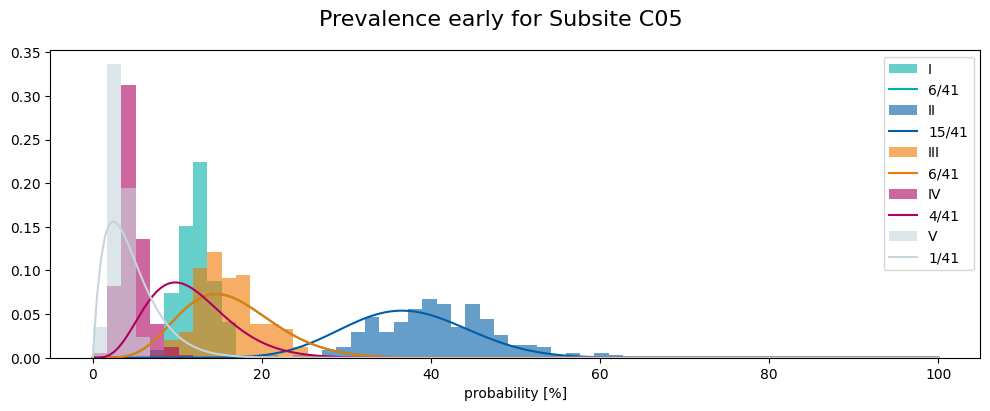
\includegraphics{figures/3_predicted_prevalence_C05_early.png}

}

\subcaption{\label{fig-oral_cavity_C05_early}}

\end{minipage}%
\newline
\begin{minipage}{\linewidth}

\centering{

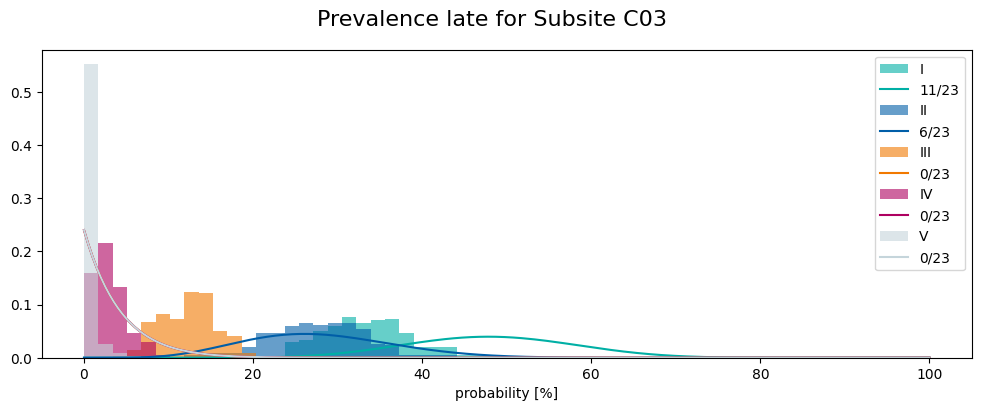
\includegraphics{figures/3_predicted_prevalence_C03_late.png}

}

\subcaption{\label{fig-oral_cavity_C03_late}}

\end{minipage}%
\newline
\begin{minipage}{\linewidth}

\centering{

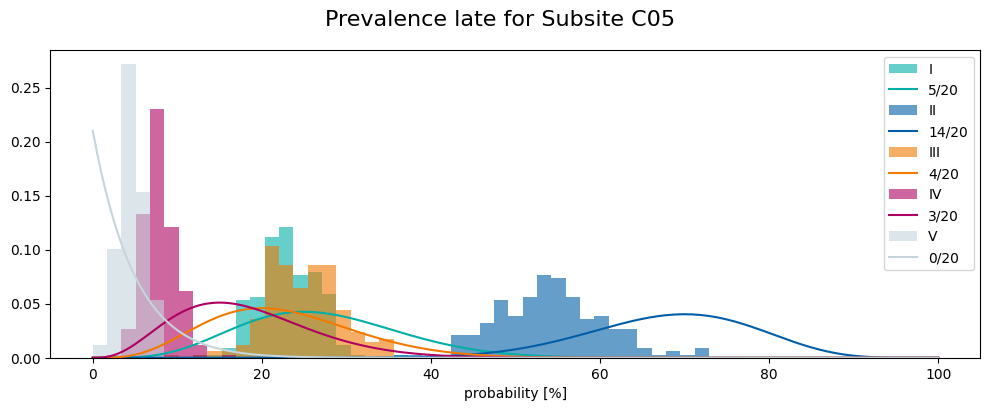
\includegraphics{figures/3_predicted_prevalence_C05_late.png}

}

\subcaption{\label{fig-oral_cavity_C05_late}}

\end{minipage}%

\caption{\label{fig-oral_cavity}Observed prevalence (solid lines) and
predicted prevalence (histograms) for subsites C03 and C05. Figures a
and b show the prevalences for early t-stages. Figures c and d show the
prevalences for late t-stages.}

\end{figure}%

In figure~\ref{fig-oropharynx} we present the predictions for the
oropharynx subsites C01 and C10. In figures
figure~\ref{fig-oropharynx_C01_early} and
figure~\ref{fig-oropharynx_C10_early} we can see that the model predicts
a higher prevalence for LNL II in subsite C01 (base of tongue) compared
to subsite C10 (oropharynx). This is consistent with the observed data.
In figures figure~\ref{fig-oropharynx_C01_late} and
figure~\ref{fig-oropharynx_C10_late} we can see that the model precisely
captures the increased prevalence in late t-stage for both subsites.
LNLs I, IV and V are predicted to have low prevalences for both
subsites, but the model does not perfectly fit the predicted prevalences
to the observed prevalences.

\begin{figure}

\begin{minipage}{\linewidth}

\centering{

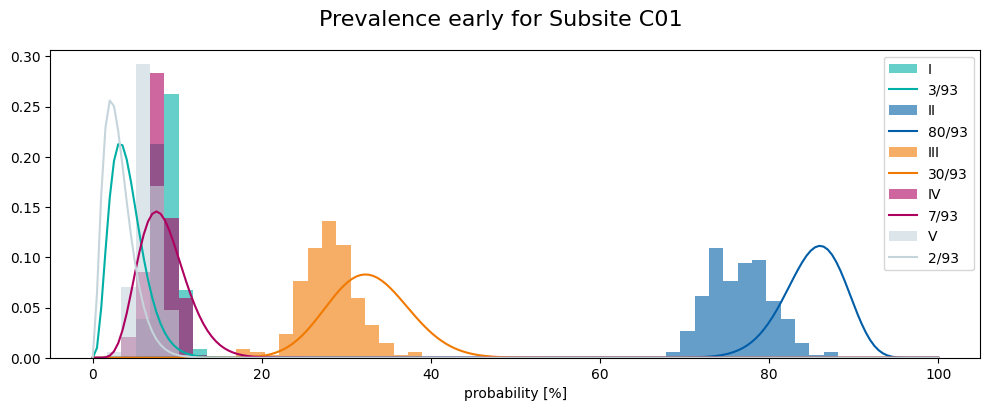
\includegraphics{figures/3_predicted_prevalence_C01_early.png}

}

\subcaption{\label{fig-oropharynx_C01_early}}

\end{minipage}%
\newline
\begin{minipage}{\linewidth}

\centering{

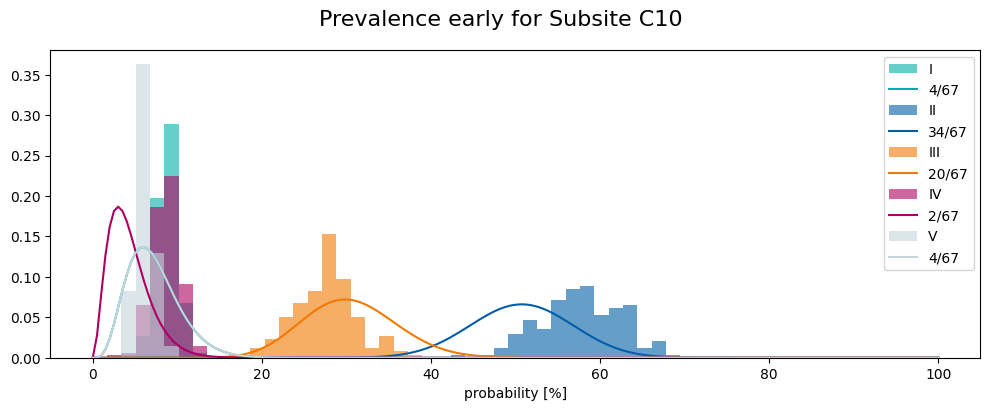
\includegraphics{figures/3_predicted_prevalence_C10_early.png}

}

\subcaption{\label{fig-oropharynx_C10_early}}

\end{minipage}%
\newline
\begin{minipage}{\linewidth}

\centering{

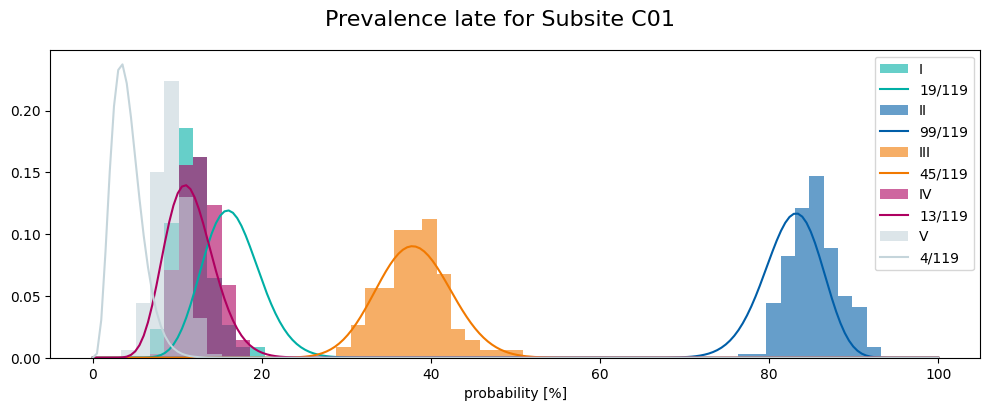
\includegraphics{figures/3_predicted_prevalence_C01_late.png}

}

\subcaption{\label{fig-oropharynx_C01_late}}

\end{minipage}%
\newline
\begin{minipage}{\linewidth}

\centering{

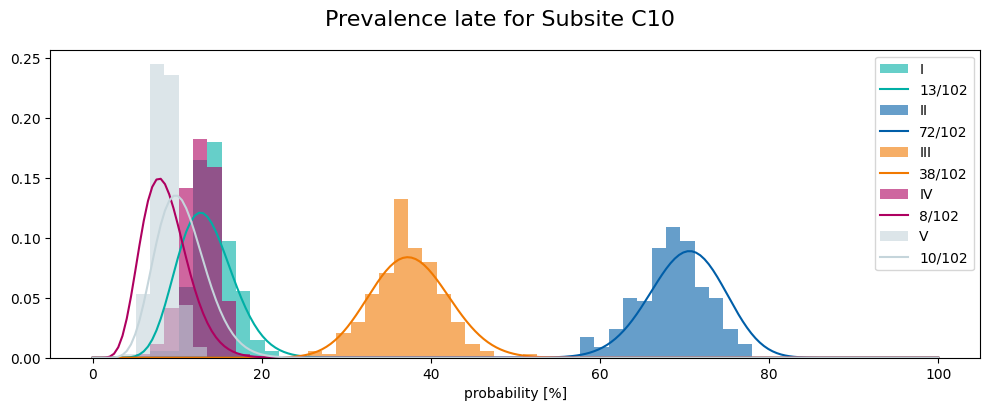
\includegraphics{figures/3_predicted_prevalence_C10_late.png}

}

\subcaption{\label{fig-oropharynx_C10_late}}

\end{minipage}%

\caption{\label{fig-oropharynx}Observed prevalence (solid lines) and
predicted prevalence (histograms) for subsites C01 and C10. Figures a
and b show the prevalences for early t-stages. Figures c and d show the
prevalences for late t-stages.}

\end{figure}%

In summary, the mixture model successfully distinguishes between
subsites, capturing the continuous variation in lymphatic spread
patterns across tumor locations. However, the model's predictions are
not always perfect. While it generally aligns with observed data,
certain nuances, such as the higher prevalence of LNL I involvement in
subsite C03 compared to C05, are not fully captured.

\subsection{Four Component Mixture Model}\label{sec-4comp}

We can extend the mixture model to include the larynx. The larynx
patients are more finely divided into ICD codes C32.0, C32.1 and C32.2
as there is a notable difference between these ICD codes in
figure~\ref{fig-involvement}.

Simlarly to the three component model, we can analyze the convergence
over the iterations of the EM-algorithm. In
figure~\ref{fig-convergence4} we can see that in this more complex
model, the likelihood space becomes more complex as at around 200
iterations, the negative log-likelihood starts to increase faster again.

\begin{figure}

\centering{

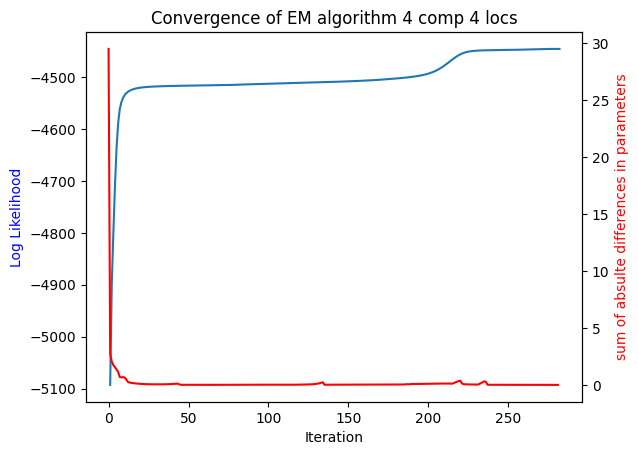
\includegraphics{figures/convergence_4_components_4_loc.png}

}

\caption{\label{fig-convergence4}The y-axis on the left shows the
negative likelihood convergence depicted in the blue line. The y-axis on
the right shows the sum of absulte difference between all model
parameters.}

\end{figure}%

The component assignment is shown in figure~\ref{fig-4-matrix}.
Similarly to the 3-component model the different tumor locations are
assigned to a one of the components. In this case, the new component is
used to model laryngeal subsites. The uncertainty of the assignments is
shown in figure~\ref{fig-4_comp_scatter_uncert}. The most striking
differences are in subsites C03 and C12, which were formerly assigned to
a single component. Now, C03 mixes with the laryngeal component, while
C12 is mixed with the laryngeal and the hypopharyngeal component.
Another interesting observation is the mixture of the supraglottis
subsite (C32.1) which is anatomically close to the hypopharynx. The
model assigns a strong mixture of the larynx-like component and the
hypopharynx-like component to this subsite. This is consistent with the
observed data, where the supraglottis subsite has a high prevalence of
LNL II and III involvement, which is also observed in the hypopharynx
subsites. In contrast, the glottis subsite (C32.0) is strongly assigned
to the laryngeal component, while the subsite C32.2 (subglottis) is
assigned to the laryngeal component with little uncertainty. This is
consistent with the observed data, where the glottis subsite has a much
lower prevalence of involvement in any LNL. However, there is a strong
t-stage dependency for this subsite.

\begin{figure}

\begin{minipage}{0.29\linewidth}

\begin{figure}[H]

\centering{

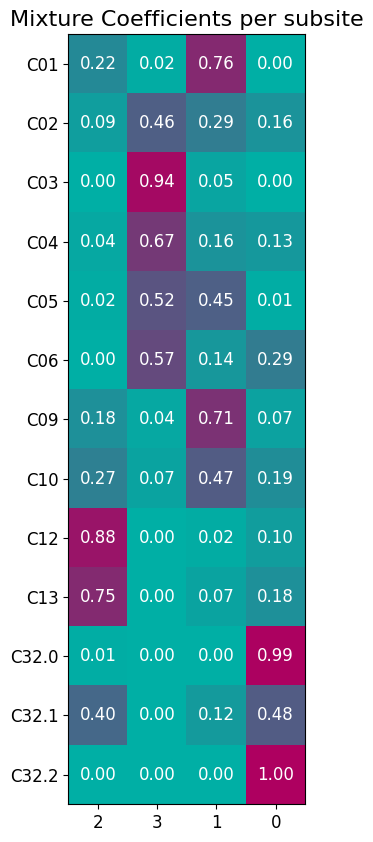
\includegraphics{figures/mixture_components_4.png}

}

\caption{\label{fig-4-matrix}Matrix representation of component
assignment. Each row of the matrix corresponds to each ICD code. The
columns represent the four different components}

\end{figure}%

\end{minipage}%
%
\begin{minipage}{0.71\linewidth}

\begin{figure}[H]

\centering{

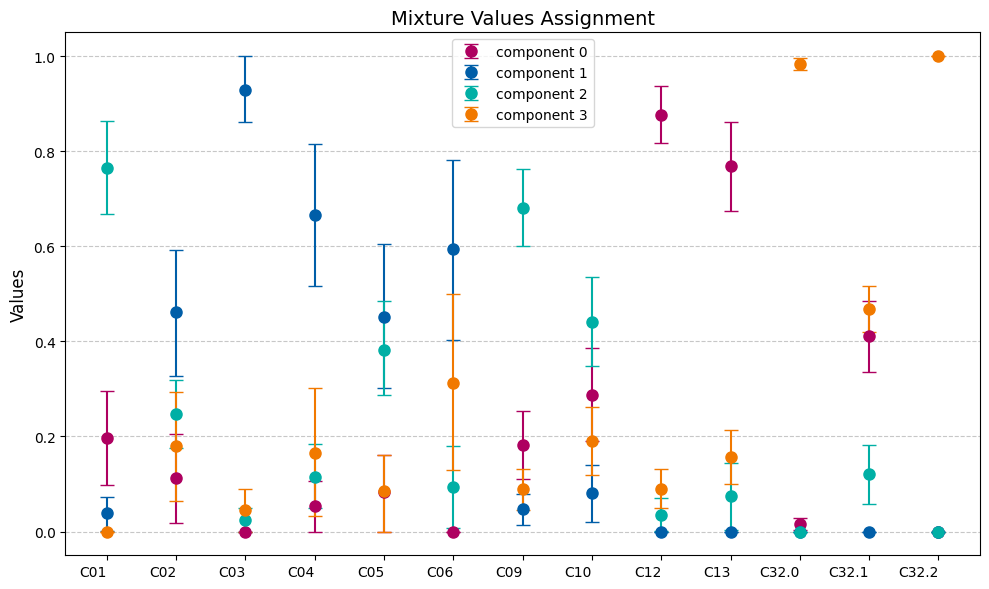
\includegraphics{figures/4_comp_mixture_coefficients_uncert_scatter.png}

}

\caption{\label{fig-4_comp_scatter_uncert}Assignment of each subsite to
each of the four components. The closer a subsite is to a vertex, the
more it is assigned to the corresponding component, with component 0 on
the bottom right, 1 on the bottom left, 2 on the top left and 3 on the
top right. The size of the marker (area) corresponds to the number of
patients in each subsite.}

\end{figure}%

\end{minipage}%

\end{figure}%

Similarly to the three component model, we can analyze the predicted and
observed prevalences for LNLs I, II, III, IV and V. We will first
revisit the oral cavity subsites C03 and C05. to check, whether the
additional component improves the model predictions. In
figure~\ref{fig-oral_cavity_4} the predictions for the oral cavity
subsites C03 and C05 are shown. The model now predicts a higher
prevalence for LNL I in subsite C03 (gum) compared to subsite C05
(palate) for both early and

\begin{figure}

\begin{minipage}{\linewidth}

\centering{

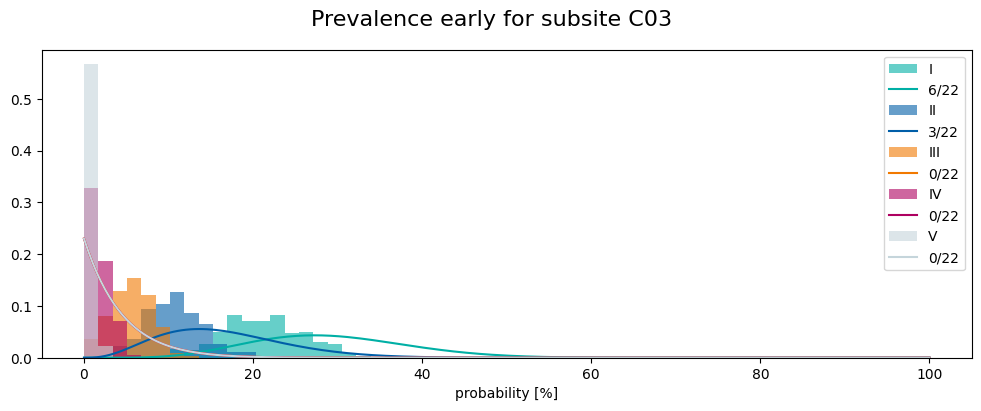
\includegraphics{figures/4_predicted_prevalence_C03_early.png}

}

\subcaption{\label{fig-oral_cavity_C03_early}}

\end{minipage}%
\newline
\begin{minipage}{\linewidth}

\centering{

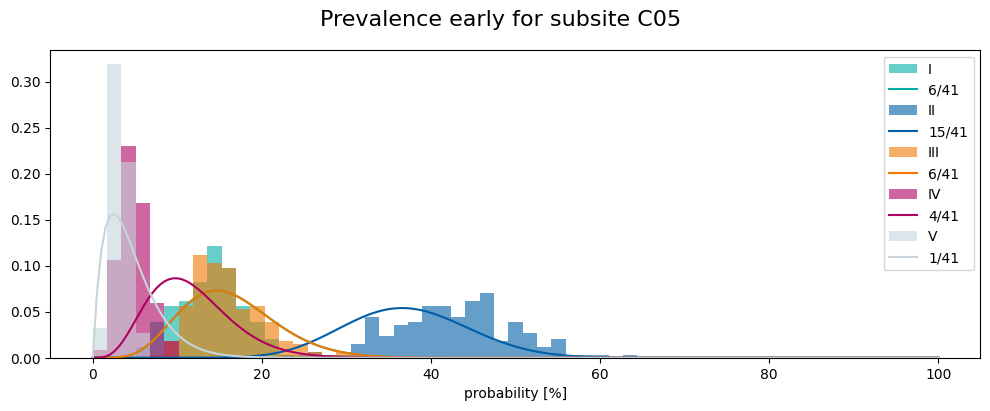
\includegraphics{figures/4_predicted_prevalence_C05_early.png}

}

\subcaption{\label{fig-oral_cavity_C05_early}}

\end{minipage}%
\newline
\begin{minipage}{\linewidth}

\centering{

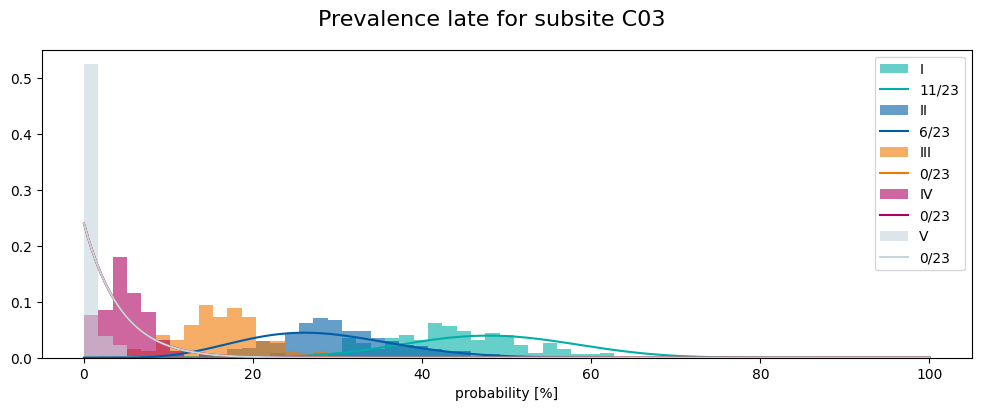
\includegraphics{figures/4_predicted_prevalence_C03_late.png}

}

\subcaption{\label{fig-oral_cavity_C03_late}}

\end{minipage}%
\newline
\begin{minipage}{\linewidth}

\centering{

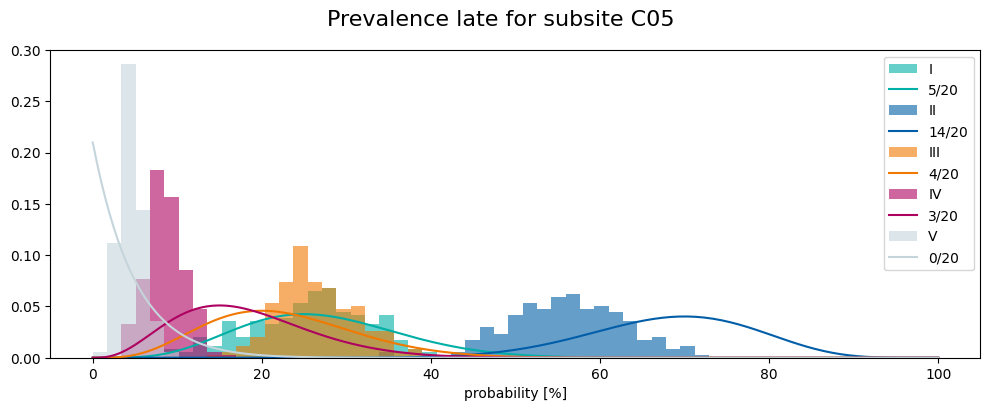
\includegraphics{figures/4_predicted_prevalence_C05_late.png}

}

\subcaption{\label{fig-oral_cavity_C05_late}}

\end{minipage}%

\caption{\label{fig-oral_cavity_4}Observed prevalence (solid lines) and
predicted prevalence (histograms) for subsites C03 and C05. Figures a
and b show the prevalences for early t-stages. Figures c and d show the
prevalences for late t-stages.}

\end{figure}%

The predicted prevalences for for the laryngeal subsites C32.0 and C32.1
are shown in figure~\ref{fig-larynx_4}. Here, the large difference
between early and late t-stages is clearly visible. For subsite C32.0
(glottis) the model predicts a very low prevalence for LNL I, II and III
in early t-stages, which is consistent with the observed data. For late
t-stages, the model captures the increased involvement probabilities for
LNLs II and III. For subsite C32.1 (supraglottis) the model
overestimates the prevalence for LNLs II and III in early t-stages and
slightly underestimates their prevalence in late t-stages.

\begin{figure}

\begin{minipage}{\linewidth}

\centering{

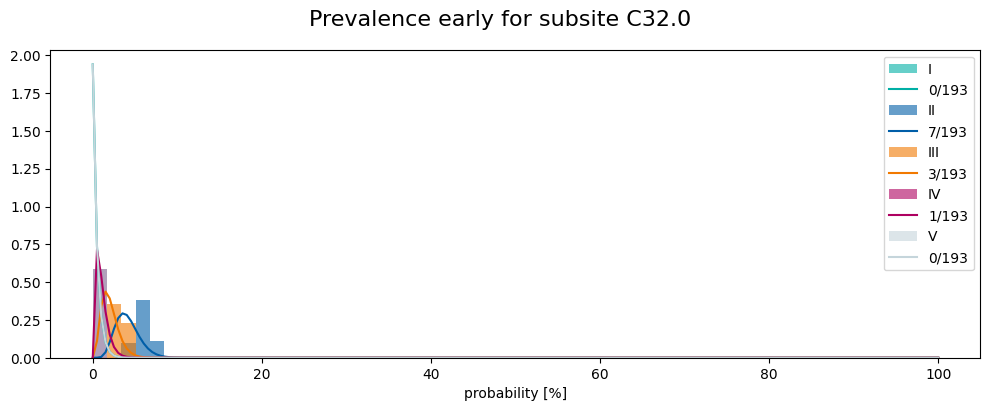
\includegraphics{figures/4_predicted_prevalence_C32.0_early.png}

}

\subcaption{\label{fig-oral_cavity_C32.0_early}}

\end{minipage}%
\newline
\begin{minipage}{\linewidth}

\centering{

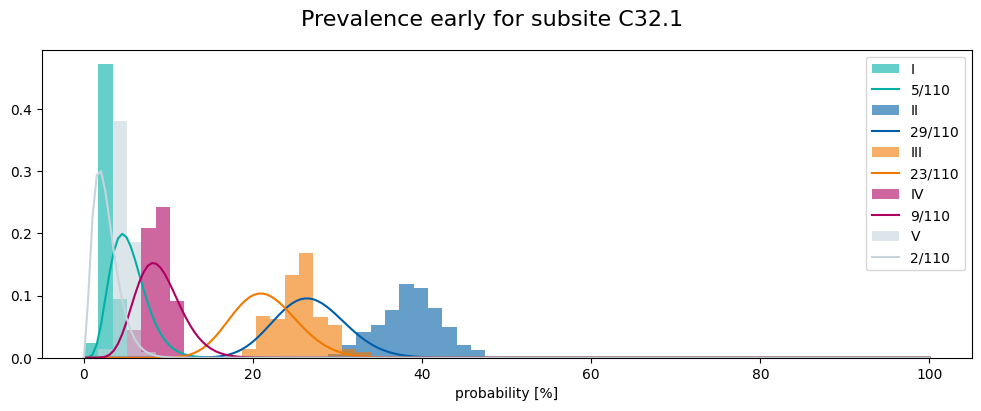
\includegraphics{figures/4_predicted_prevalence_C32.1_early.png}

}

\subcaption{\label{fig-oral_cavity_C05_early}}

\end{minipage}%
\newline
\begin{minipage}{\linewidth}

\centering{

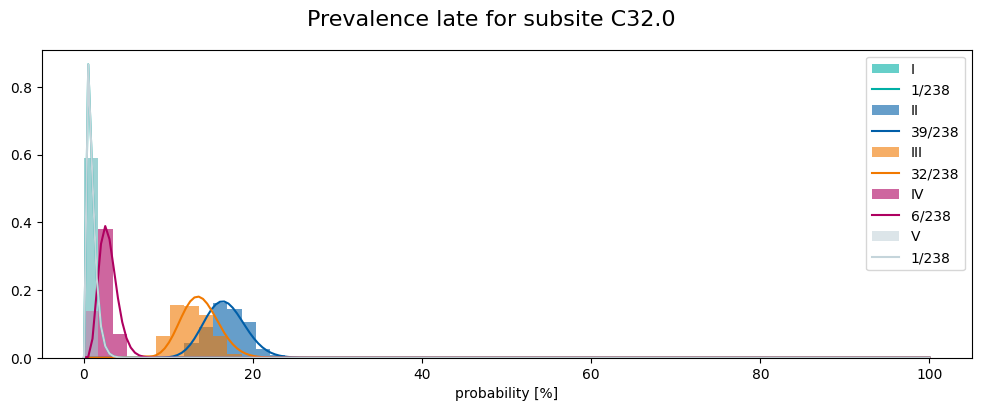
\includegraphics{figures/4_predicted_prevalence_C32.0_late.png}

}

\subcaption{\label{fig-oral_cavity_C03_late}}

\end{minipage}%
\newline
\begin{minipage}{\linewidth}

\centering{

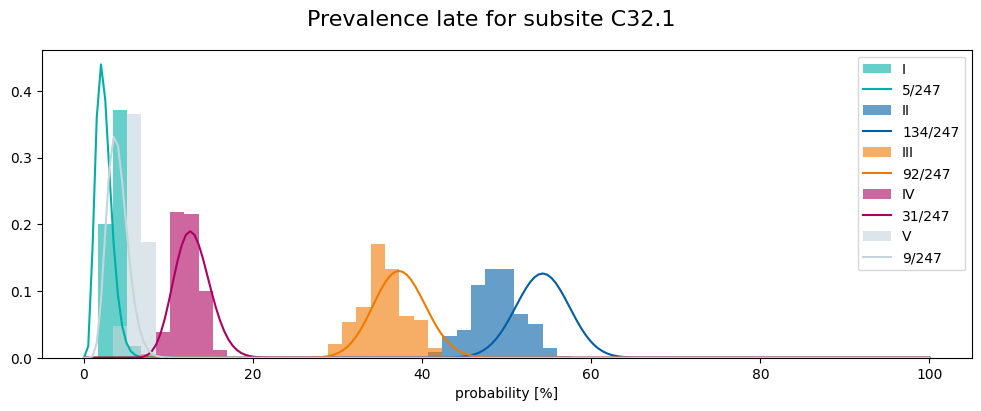
\includegraphics{figures/4_predicted_prevalence_C32.1_late.png}

}

\subcaption{\label{fig-oral_cavity_C05_late}}

\end{minipage}%

\caption{\label{fig-larynx_4}Observed prevalence (solid lines) and
predicted prevalence (histograms) for subsites C32.0 and C32.1. Figures
a and b show the prevalences for early t-stages. Figures c and d show
the prevalences for late t-stages.}

\end{figure}%

The model parameters for the larynx-like component are shown in
figure~\ref{fig-4_larynx_parameters}. The parameter that governs the
impact of t-stage \(p_late\) is estimated around 1. Therefore, the model
maximizes the increase of risk of involvement for late t-stages to
capture the large difference in prevalence between early and late
t-stages.

\begin{figure}

\centering{

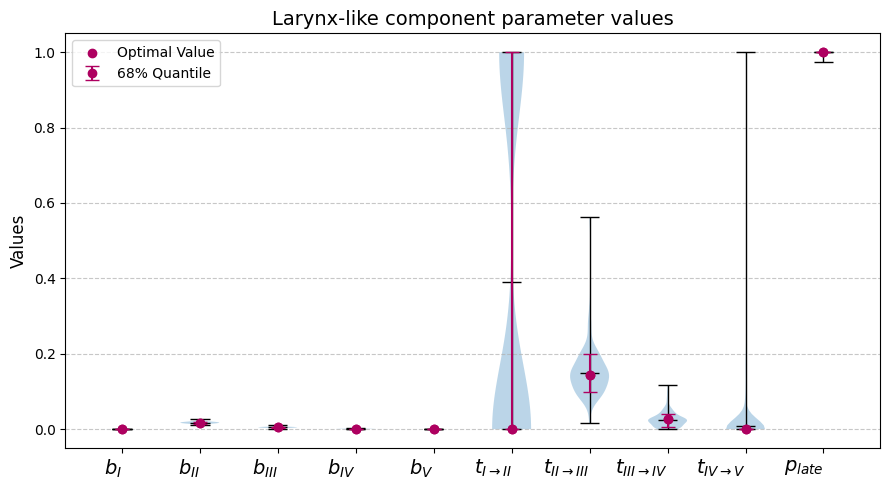
\includegraphics{figures/larynx_component_values.png}

}

\caption{\label{fig-4_larynx_parameters}Model parameters for the
larynx-like component. The optimal value and the 68\% percentile around
the optimal value are marked in red. The mean values and extreme values
are indicated by the black bars.}

\end{figure}%

\section{Model Predictions}\label{sec-model_pred}

Given the model parameters, we can compute the risk of occult metastases
given a patient's diagnosis. The model can be applied to predict the
risk of involvement for each LNL, given the patient's t-stage and
primary tumor subsite.

The risk predictions are computed by applying the equation~\ref{eq-risk}
to each component and subsequently mixing the results using the mixture
coefficients \(\boldsymbol{\pi}\). The risk of involvement for each LNL
\(v\) in subsite \(s\) is given by:
\begin{equation}\phantomsection\label{eq-risk-mixing}{
P(X_v^s=1 \mid \mathbf{D}, \boldsymbol{\theta}) = \sum_{m=1}^M \pi_m^{s} P(X_v=1 \mid \mathbf{D}, \boldsymbol{\theta}_m)
}\end{equation}

where \(s\) is the subsite and \(\boldsymbol{\theta}_m\) are the
parameters of model component \(m\).

For all estimates we will set a 5\% threshold for the risk of
involvement. This means that if the model predicts a risk of involvement
of 5\% or higher, we will consider the LNL to be at a ``high'' risk of
involvement and should be irradiated. Consequently all LNLs with a risk
of involvement below 5\% will be considered to be at a ``low'' risk of
involvement and should not be irradiated. This allows us to compare the
model predictions with the current clinical guidelines for elective
irradiation of LNLs.

In the following sections we will analyze the model predictions for the
four component model only and for selected clinical diagnoses.

\subsection{Oral cavity}\label{oral-cavity}

Oral cavity tumors typically spread to LNLs I, II and III as shown in
figure~\ref{fig-involvement}. Consequently, the clinical guidelines
recommend irradiating LNLs I, II, III for all tumors, irrespective of
t-stage and even if there is no LNL involvement
\citep{biau_selection_2019}.

We first analyze the risk predictions for the case where we clinically
diagnose no positive LNLs

\begin{figure}

\begin{minipage}{0.50\linewidth}

\centering{

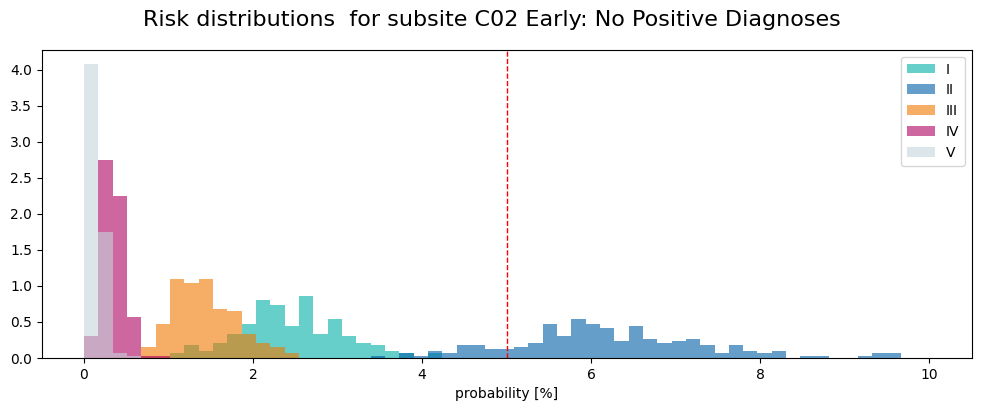
\includegraphics{figures/plot_C02_early_no_positive_diagnoses.png}

}

\subcaption{\label{fig-oral_cavity_no_pos_C02_early}}

\end{minipage}%
%
\begin{minipage}{0.50\linewidth}

\centering{

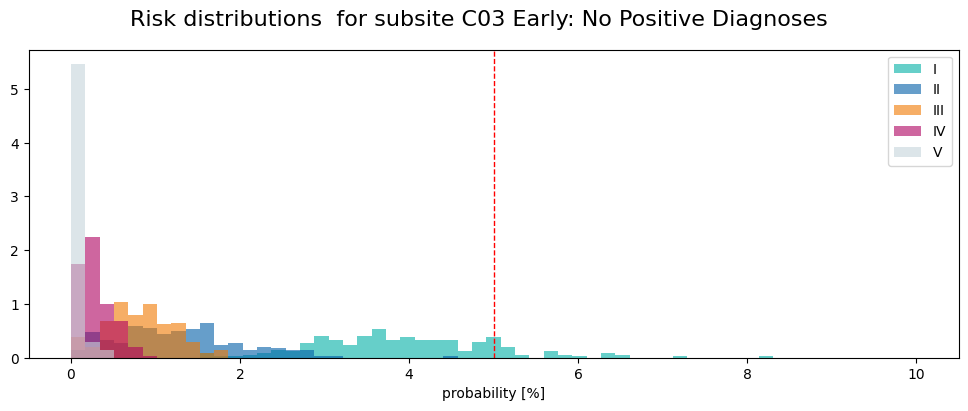
\includegraphics{figures/plot_C03_early_no_positive_diagnoses.png}

}

\subcaption{\label{fig-oral_cavity_no_pos_C03_early}}

\end{minipage}%
\newline
\begin{minipage}{0.50\linewidth}

\centering{

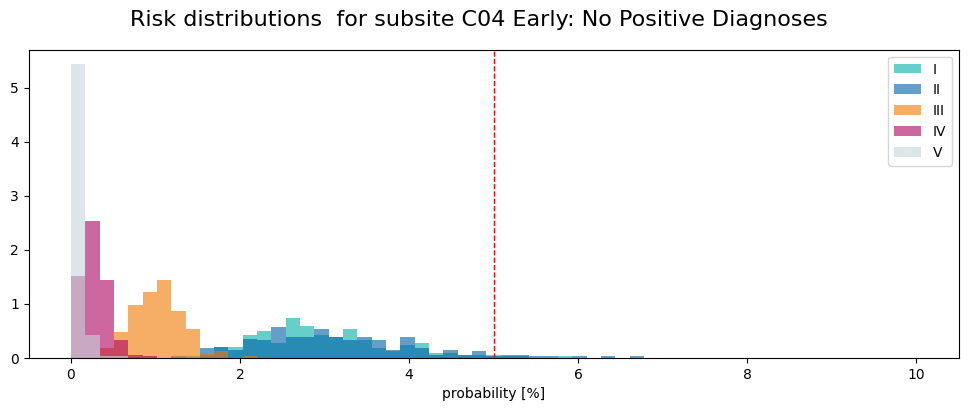
\includegraphics{figures/plot_C04_early_no_positive_diagnoses.png}

}

\subcaption{\label{fig-oral_cavity_no_pos_C04_early}}

\end{minipage}%
%
\begin{minipage}{0.50\linewidth}

\centering{

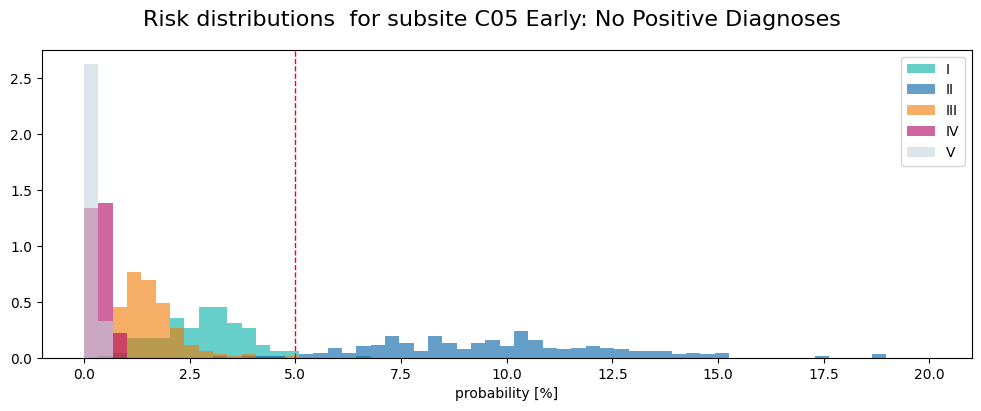
\includegraphics{figures/plot_C05_early_no_positive_diagnoses.png}

}

\subcaption{\label{fig-oral_cavity_no_pos_C05_early}}

\end{minipage}%
\newline
\begin{minipage}{0.50\linewidth}

\centering{

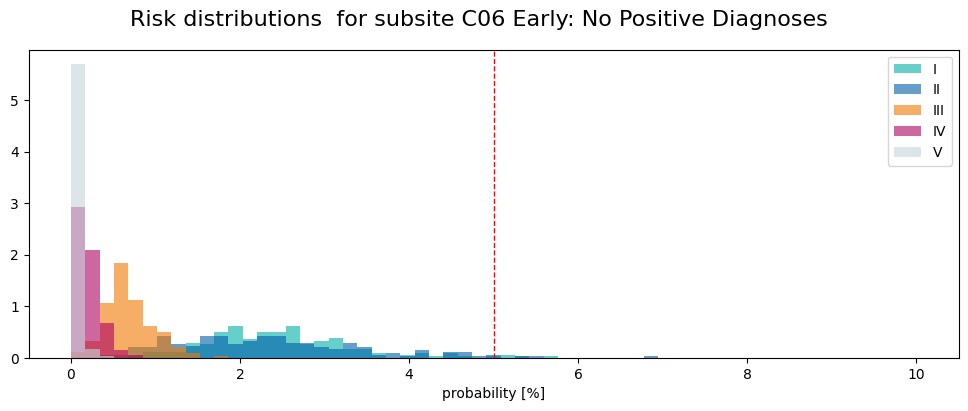
\includegraphics{figures/plot_C06_early_no_positive_diagnoses.png}

}

\subcaption{\label{fig-oral_cavity_no_pos_C06_early}}

\end{minipage}%

\caption{\label{fig-oral_cavity_early_no_pos}Probability of occult
metastases in LNLs I, II, III, IV and V for early t-stages in oral
cavity subsites C02 (tongue), C03 (gum), C04 (floor of mouth), C05
(palate) and C06 (other parts of mouth). The red line marks the 5\%
threshold for high risk of involvement.}

\end{figure}%

In figure~\ref{fig-oral_cavity_early_no_pos} we can see that the model
predicts different risks of involvement for each subsite. For subsite
C03 (gum), predicts a higher risk of involvement for LNL I. In subsites
C02 (tongue) and C05 (palate), the model predicts an above threshold
risk of involvement for LNL II. While for subsites C02 (tongue) and C06
(other parts of mouth) all LNLs stay below the 5\% threshold. Thus, the
model would propose three different treatment plans for these subsites,
with C03 (gum) LNL I, C02 (tongue) LNL II and C05 (palate) LNL II being
irradiated, while C04 (floor of mouth) and C06 (other parts of mouth)
would not need elective irradiation at all, which is a major deviation
from the clinical guidelines which irradiate LNLs I, II and III for all
oral cavity subsites.

\section{Appendix}\label{appendix}

Here I will probably add more figures such as all component parameter
estimates and their uncertainties.


  \bibliography{references.bib}



\end{document}
